\documentclass[11pt]{article}
\usepackage[margin=0.9in]{geometry}
\usepackage[T1]{fontenc}
\usepackage{lmodern,microtype}
\usepackage{amsmath,amssymb,amsthm,mathtools}
\usepackage{booktabs,tabularx,array}
\usepackage{xcolor,graphicx,adjustbox,placeins}
\usepackage[numbers,sort&compress]{natbib}
\usepackage[colorlinks=true,linkcolor=blue!45!black,citecolor=blue!45!black,urlcolor=blue!45!black]{hyperref}
\usepackage{enumitem}
\setlist{nosep}
\newtheorem{theorem}{Theorem}
\newtheorem{proposition}[theorem]{Proposition}
\newtheorem{corollary}[theorem]{Corollary}
\theoremstyle{definition}
\newtheorem{definition}[theorem]{Definition}
\newcommand{\R}{\mathbb R}
\newcommand{\sg}{\operatorname{sigmoid}}
\newcommand{\spplus}{\operatorname{softplus}}
\newcommand{\clip}{\operatorname{clip}_{[0,1]}}
\newcommand{\diag}{\operatorname{diag}}
\newcommand{\bdiag}{\operatorname{blockdiag}}
\newcommand{\Had}{\odot}
\newcommand{\norm}[1]{\left\lVert #1\right\rVert}
\newcommand{\sech}{\operatorname{sech}}
\newcommand{\measured}[1]{\IfFileExists{results/generated.tex}{#1}{\textit{[measured; filled from the reproduction records]}}}
\title{Experience as a Persistent Object:\\Online Temporal Credit in DABSN}
\author{Nicholas Rosdahl\\Independent Researcher}
\date{November 2026\\[0.5em]\small\href{https://doi.org/10.5281/zenodo.24268687}{doi:10.5281/zenodo.24268687}}

\begin{document}
\maketitle

\begin{abstract}
What remains of an experience after its computation graph is gone? In DABSN,
online temporal credit carries an architecture-defined object $E$ across every
boundary at which the recurrent state is carried. Its later operations are not
fixed by the objective used to inspect it. We specify $E$ exactly. Each of the
four dense matrices keeps one trace per entry, on the baseline (budget) channel
of the unit that owns it. Each of the sixteen per-unit controls and the four
shared controls keeps a trace on all three state channels: baseline, energy and
saturation. For input width $I$, state width $S$ and $B$ stream lanes, $E$ holds
exactly $B(2SI+2S^2+60S)$ scalars, independent of elapsed history and about the
size of the parameter vector, while full real-time sensitivity needs
$3BS(2SI+2S^2+16S+4)$. We prove composition across arbitrary contiguous
partitions at fixed parameters and an exact identity for the influence $E$
omits. We then show that $E$ is a different function of experience from both
the predictive state and the full terminal state--parameter Jacobian: histories
with identical weights and predictive states can require opposite credit, and an
explicit construction gives histories with the same full terminal Jacobian but
different $E$, and histories with the same $E$ but different terminal Jacobians.
The same object supplies a response geometry whose Gram matrix is block diagonal
by unit up to a rank-four shared correction, response scales without persistent
optimizer moments, regularized direct parameter action, and causal edits under
unchanged forward computation. A locked, resumable reproduction tests these
operations together with matched delayed learning against full BPTT and a
frozen-core control, learning on uninterrupted streams (memory capacity and NARMA-10), objective-conditioned
continuation, a bounded characterization of what $E$ encodes, and continuity with
DABSN's architecture results. With one chunk per episode, online credit matches
full BPTT on the adding and temporal order problems at every evaluated length,
while a frozen core stays at chance. At a frozen checkpoint, erasing $E$ one step
before the query removes most of the core's credit under unchanged forward
computation. Driven by $E$ alone, with credit, direction and pace from $E$ and no
optimizer state, the core matches AdamW with online credit and with BPTT on copy,
MQAR and key--value recall, and on uninterrupted streams it outperforms Adam acting
on the same credit. Two limits are measured: on A5/60, where the same model trained
by BPTT is exact at every length to 64 times its training length, online credit is
not, a cost of the influence $E$ omits; and on uninterrupted streams, truncated BPTT
over a 64-step window remains far stronger than any arm that learns through $E$.
\end{abstract}

\section{Introduction}

An experience changes what a continuing system can do. It changes what the system
predicts, which parameters a later signal addresses, and which responses become
available when the purpose of the experience is specified afterward. These effects
need not live in one representation. A predictive state can preserve an event
after its computation graph is gone; conversely, two experiences can leave the
same predictive state while demanding different parameter actions. The object
that survives an experience therefore matters independently of the output the
experience produced.

DABSN makes this distinction operational. Its online temporal-credit mechanism
carries an object $E$ across the same stream boundaries as the recurrent state
\citep{rosdahl2026dabsn}. The history need not remain available as a sequence of
differentiable activations. A later learning signal is contracted with $E$ to
address past parameter involvement. That contraction is one operation on the
object; its columns also define response magnitudes and relationships among
parameters that other readouts use directly. The central question is what this
persistent object represents and what it enables.

The question matters for models meant to run continuously. Backpropagation through
time (BPTT) represents temporal dependence through a retained or recomputed graph
\citep{werbos1990bptt}. Real-time recurrent learning (RTRL) carries the full
sensitivity of state to parameters \citep{williams1989rtrl}, whose size grows
with the product of state and parameter counts. Eligibility-based methods choose
other ways to preserve historical influence; their representations, learning
signals and structural assumptions decide what a delayed loss can change
\citep{murray2019rflo,bellec2020eprop,bohnstingl2023ostl,marschall2020unified}.

DABSN's persistent-modulation core offers a specific design opportunity. It
separates an expressed activation from a persistent baseline, an energy state and
a saturation state \citep{rosdahl2026dabsn}. These variables play different roles:
the baseline is where a write lands, while energy and saturation regulate when and
how strongly a write occurs. The online rule assigns historical traces by role.
Each matrix entry keeps the history of its effect on the baseline of the unit it
writes into. Each control keeps the history of its effect on all three channels.
The result is one trace per matrix entry plus sixty scalars per unit: an object the
size of the parameter vector.

The implemented storage is called eligibility, but the name does not settle its
information content. We identify $E$ by its recurrence and its observable
operations. This allows a stronger question than agreement with one gradient: can
$E$ distinguish experiences that the full terminal state--parameter Jacobian
identifies? An explicit construction answers yes, and a second construction
establishes the converse. The relationship between the two objects is a matter of
what they record about histories, not only of how numerically close their readouts
are.

The argument has three parts. First, we specify the object exactly: its role
allocation, transport, direct sources, storage and native contraction
(Section~\ref{sec:method}). Second, we prove what it guarantees and what
distinguishes it: partition composition, an exact account of omitted influence,
predictive-state collisions, bidirectional separation from full terminal
sensitivity, and a channelwise response geometry (Sections~\ref{sec:theory}
to~\ref{sec:operator}). Third, we test the operations that follow, under one locked
and resumable protocol: learning after graph boundaries, causal edits of $E$ at
frozen checkpoints, learning on uninterrupted streams, signals selected after
experience, objective-conditioned continuation, direct parameter action, learning
driven by $E$ alone, and a bounded characterization of what $E$ encodes
(Section~\ref{sec:validation}).

The subject is the online rule of the DABSN core. The architecture paper studies
the full block and its empirical behavior \citep{rosdahl2026dabsn}. Separating the
core from its read bank and surrounding modules makes the learning object
identifiable. The theorems concern that object; claims about language modeling,
throughput or comparative model quality require their own experiments.

\section{Experience, persistent state, and derivative readouts}
\label{sec:objects}

Let inputs $x_t\in\R^I$ be prescribed independently of the core parameters
$\theta\in\R^P$. Write the recurrent transition and its emitted signals as
\begin{equation}
 s_{t+1}=F_\theta(s_t,x_t),\qquad o_t=O_\theta(s_t,x_t).
 \label{eq:system}
\end{equation}
At differentiable points define
\begin{equation}
 J_t=\partial_sF_\theta(s_t,x_t),\quad
 U_t=\partial_\theta F_\theta(s_t,x_t),\quad
 H_t=\frac{\partial s_t}{\partial\theta}.
 \label{eq:derivatives}
\end{equation}
For a parameter-independent initial state, $H_0=0$ and exact sensitivity obeys
\begin{equation}
 H_{t+1}=J_tH_t+U_t.
 \label{eq:rtrl}
\end{equation}
This is the RTRL recurrence. A state of dimension $D$ carries a $D\times P$
sensitivity, before any architectural structure is used.

Let $v_t$ be a cotangent on $o_t$, for example the derivative of a loss with
respect to that emitted signal, held fixed when credit computations are compared.
The exact current-step derivatives are
\begin{equation}
 \delta_t=(\partial_s O_\theta)^\top v_t,\qquad
 d_t=(\partial_\theta O_\theta)^\top v_t,
 \label{eq:local-vjp}
\end{equation}
and the core parameter gradient for these signals is
\begin{equation}
 g=\sum_{t=0}^{T-1}\left(d_t+H_t^\top\delta_t\right).
 \label{eq:full-gradient}
\end{equation}
The first term accounts for the parameter's current use, the second for its
influence on the incoming state. The timing matters: the historical term contracts
$H_t$ before the sensitivity advances to $H_{t+1}$.

An online credit rule instead specifies a compact state $e_t$, a transport
$e_{t+1}=\mathcal T_t(e_t)$, and a contraction that adds historical credit to
$d_t$. Calling the state an eligibility does not decide whether it equals a full
derivative, an estimator, a selected sensitivity or some other representation.
Its update must make that precise.

\section{The persistent object $E$}
\label{sec:method}

\subsection{The forward substrate}

Use channel-major state
\begin{equation}
 s_t=((b_{t,i},e_{t,i},q_{t,i}))_{i=1}^S\in\R^{3S},
\end{equation}
where $b$ is the persistent baseline (\texttt{budget} in the implementation), $e$
the energy available for plasticity and $q$ the saturation. The core forms
\begin{align}
 y_t&=\tanh(Wx_t+b_t), & a_t&=Ay_t,\\
 z_t&=W_gx_t+U_gy_t+c, & g_t&=\operatorname{hardsigmoid}(z_t),\\
 n_t&=\tanh(|a_t-b_t|), & p_t&=g_t\Had e_t,
 \label{eq:forward-core}
\end{align}
and updates its baseline by
\begin{equation}
 b_{t+1}=(1-\alpha)b_t+\beta+\lambda(p_t\Had a_t).
 \label{eq:budget}
\end{equation}
Energy and saturation regulate this write through nonlinear transitions given in
Appendix~\ref{app:recurrence}. $W,W_g\in\R^{S\times I}$ and $A,U_g\in\R^{S\times S}$
are ordinary dense matrices, and the forward core keeps their full products. The
credit rule below is channel-local in its transport; it does not diagonalize the
forward computation.

The emitted core signals are
\begin{equation}
 o_t=(y_t,b_{t+1},n_t,p_t,a_t,p_t\Had a_t,e_t,q_{t+1}).
 \label{eq:signals}
\end{equation}
Their current-step vector--Jacobian products use the full dense spatial
derivatives; in particular the local backward computation includes $A^\top$ and
$U_g^\top$. The energy signal is incoming energy and the saturation signal is
outgoing saturation.

\subsection{A representation chosen by parameter role}
\label{sec:projection}

Let $D_t=\bdiag(J_{t,11},\ldots,J_{t,SS})$ keep the $3\times3$ within-unit blocks
of $J_t$: each unit's next baseline, energy and saturation differentiated with
respect to its own entering state, through its own $y$ and the diagonal entries
$A_{ii}$ and $U_{g,ii}$. Split the parameters into the matrix families
$\mathcal M=\{W,A,W_g,U_g\}$, the sixteen per-unit controls $\mathcal L$, and the
four shared controls $\mathcal G$ (Appendix~\ref{app:recurrence}). Each parameter
coordinate has an owner: the row unit of a matrix entry, the unit of a per-unit
control, or every unit for a shared control. Let $\Pi$ be the role mask on the
$3S$ state coordinates of each parameter column:
\begin{itemize}
 \item matrix entries keep only their owner's baseline coordinate;
 \item per-unit controls keep their owner's three coordinates;
 \item shared controls keep all coordinates.
\end{itemize}
The embedded learning operator obeys
\begin{equation}
 \boxed{K_{t+1}=\Pi\Had\big(D_tK_t+U_t\big),\qquad K_0=0.}
 \label{eq:online}
\end{equation}
For a matrix entry $\theta_{ij}$ this is a scalar recurrence,
\begin{equation}
 E^{\theta}_{t+1,ij}=j^{bb}_{t,i}\,E^{\theta}_{t,ij}+u^{\theta}_{t,ij},\qquad
 j^{bb}_{t,i}=\frac{\partial b_{t+1,i}}{\partial b_{t,i}},
 \label{eq:matrix-trace}
\end{equation}
where $u^\theta_{t,ij}=\partial b_{t+1,i}/\partial\theta_{ij}$ is the direct source
on the owner's baseline:
\begin{align}
 u^{W}_{ij}&=\lambda e_i(1-y_i^2)\,x_j\,\big(a_i\,h'(z_i)\,U_{g,ii}+g_iA_{ii}\big), &
 u^{A}_{ij}&=\lambda e_ig_i\,y_j,\\
 u^{W_g}_{ij}&=\lambda e_ia_i\,h'(z_i)\,x_j, &
 u^{U_g}_{ij}&=\lambda e_ia_i\,h'(z_i)\,y_j,
 \label{eq:sources}
\end{align}
with $h'$ the hard-sigmoid slope. Per-unit and shared controls advance their
three-channel traces by the owner's $3\times3$ block $J_{t,ii}$ plus their direct
sources. Every coordinate of the stored object is therefore one of the following:
\begin{align}
 E^W,E^{W_g}&\in\R^{B\times S\times I}, &
 E^A,E^{U_g}&\in\R^{B\times S\times S},\\
 E^{\rm local}&\in\R^{B\times S\times3\times16}, &
 E^{\rm shared}&\in\R^{B\times S\times3\times4}.
\end{align}
This is a family-dependent recurrence, not a projection of a completed RTRL
history. In the implementation these are the tensors \texttt{w\_budget},
\texttt{a\_budget}, \texttt{wg\_budget}, \texttt{ug\_budget}, \texttt{local} and
\texttt{global\_} of \texttt{CoreEligibilityState}.

The native readout uses the incoming-state signal of
Eq.~\eqref{eq:local-vjp}:
\begin{equation}
 \widehat g=\sum_t\big(d_t+K_t^\top\delta_t\big).
 \label{eq:readout}
\end{equation}
For $W_{ij}$ the historical contribution is $\sum_b\delta^{b}_{b,i}E^W_{b,ij}$,
where $\delta^b$ is the baseline component of the incoming-state signal. Readout
precedes advancement. Current-event direct credit and local input credit stay
separate; the latter carries no historical input Jacobian to preceding
components.

\section{What the representation guarantees}
\label{sec:theory}

\subsection{History-independent persistent storage}
\label{sec:storage}
\begin{proposition}[Allocated learning-state size]
\label{prop:storage}
For the stated dense core, $P=2SI+2S^2+16S+4$ and $E$ contains
\begin{equation}
 N_E=B\,(2SI+2S^2+60S)
 \label{eq:storage}
\end{equation}
scalars, independent of the number of elapsed events.
\end{proposition}
\begin{proof}
The six tensors contribute $BSI$, $BS^2$, $BSI$, $BS^2$, $48BS$ and $12BS$
entries.
\end{proof}
Per lane, $N_E/B=P+44S-4$: one trace per parameter plus $44S-4$ further scalars
for the controls' energy and saturation channels. The full dense sensitivity has
$3SP$ entries per lane, so for $I=S$ the full object is larger by a factor that
grows linearly with width (Table~\ref{tab:storage}). This is an allocation count,
not a throughput claim. Physical state, read memory, optimizer moments,
current-chunk tapes and temporary buffers are separate allocations, measured
separately in Section~\ref{sec:resource}.

\begin{table}[t]
\centering\small
\caption{Exact per-lane counts for $I=S$ (FP32 sizes). The reproduction checks the
formula against actual allocations at small shapes; large widths are computed from
the formula, never allocated.}
\label{tab:storage}
\begin{tabular}{rrrrr}
\toprule
$S$ & parameters $P$ & $E$ scalars & full sensitivity $3SP$ & ratio\\
\midrule
16 & 1,284 & 1,984 & 61,632 & 31.1\\
64 & 17,412 & 20,224 & 3,343,104 & 165.3\\
256 & 266,244 & 277,504 & 204,475,392 & 736.8\\
1024 & 4,210,692 & 4,255,744 & 12,935,245,824 & 3039.5\\
4096 & 67,174,404 & 67,354,624 & 825,439,076,352 & 12255.1\\
\bottomrule
\end{tabular}
\end{table}

\subsection{Composition across detached boundaries}
\label{sec:composition}
\begin{theorem}[Partition composition]
\label{thm:partition}
Fix parameters, inputs, the initial physical state and $E$, and the emitted-signal
cotangents. Advancing Eq.~\eqref{eq:online} over any contiguous partition of the
history gives the same final object and the same summed credit in exact
arithmetic.
\end{theorem}
\begin{proof}
Each family obeys an affine update in $K$ whose coefficients depend only on the
physical trajectory. Composition of affine maps is associative, and the readout is
linear in the entering object with the same current-event term at each event.
Carrying both physical and learning state preserves the event-by-event
calculation regardless of where boundaries fall.
\end{proof}
Floating-point implementations test numerical agreement. Changing weights between
chunks, reordering updates or changing learning signals falls outside this
fixed-parameter theorem. Under changing weights, $E$ records the transitions
actually used, not the full-history derivative under the latest weights. Stream
identity is part of the contract: each lane's object belongs to its own history.

\subsection{An exact account of omitted influence}
\label{sec:residual}
\begin{theorem}[Residual identity]
\label{thm:residual}
Let $\Delta_t=H_t-K_t$. Then
\begin{equation}
 \Delta_{t+1}=J_t\Delta_t+(J_t-D_t)K_t+(1-\Pi)\Had\big(D_tK_t+U_t\big),
 \qquad g-\widehat g=\sum_t\Delta_t^\top\delta_t .
 \label{eq:residual}
\end{equation}
\end{theorem}
\begin{proof}
Subtract Eq.~\eqref{eq:online} from Eq.~\eqref{eq:rtrl} and write
$J_tH_t=J_t\Delta_t+J_tK_t$. The credit identity follows from
Eqs.~\eqref{eq:full-gradient} and~\eqref{eq:readout}, whose current-step terms
coincide.
\end{proof}
The two driving terms are the whole of what the rule omits. $(J_t-D_t)K_t$ is
cross-unit transport through the off-diagonal entries of $A$ and $U_g$.
$(1-\Pi)\Had(D_tK_t+U_t)$ is the matrix families' energy and saturation history and
their cross-unit direct sources. Control columns satisfy $\Pi=1$ on their support,
so for them only the cross-unit transport term remains; in a single unit
($J_t=D_t$) control credit is exact. The identity gives an exact account of the
difference between $E$ and full sensitivity. It does not claim that a small
instantaneous difference implies equal optimization trajectories.

\begin{proposition}[Scalar omitted influence]
\label{prop:scalar}
Take a one-unit core ($I=S=1$) with every parameter zero except $A=1$,
$\beta=\tfrac12\log3$, $\alpha=\tfrac12$, $\lambda=1$, write cost $\kappa=\tfrac1{10}$,
recovery $\rho=\tfrac1{10}$ and $k_y=1$, started from the default state $(0,1,0)$.
After the input history $(1,0)$ the boundary state is $b=\tfrac12\log3$ (so $y=\tfrac12$)
and $e=\tfrac{19}{20}$, and the derivative of the final baseline with respect to $W$
at $W=0$ is $27/64$, while the online rule gives $137/320$. The difference, $-1/160$, is exactly the omitted
energy pathway $j^{be}\,u^{W,e}=\tfrac14\cdot(-\tfrac1{40})$. Negating the first
input leaves every forward value unchanged and negates both credits. The
log-cost control's online credit equals its exact credit, $-(1-e^{-1/10})/8$.
\end{proposition}
\begin{proof}
Exact rational evaluation of Eq.~\eqref{eq:matrix-trace} and Eq.~\eqref{eq:rtrl}
for this core; the reproduction verifies each value in exact arithmetic
(\texttt{proofs/residual.py}) and against framework autograd and central finite
differences (\texttt{oracles/counterexample}).
\end{proof}
The negated history is a \emph{predictive-state collision}: identical weights,
identical predictive trajectories, opposite required credit. Equal current
computation does not imply equal subsequent credit, so no function of the
predictive state alone can serve as the credit state.

\begin{proposition}[Erased isolated historical pathway]
\label{thm:delayed}
If loss-connected current inputs are zero and the entering object is erased, the
current plus historical credit to $W$ is zero.
\end{proposition}
\begin{proof}
Current-event $W$ credit is proportional to its current input, and the historical
term contracts the zero entering $W$ trace.
\end{proof}

\section{Separating information from credit}
\label{sec:separation}

Predictive state, full terminal sensitivity and $E$ are different functions of
history. A one-unit construction establishes both directions of the
terminal-sensitivity distinction for the rule of Eq.~\eqref{eq:online}.

Set $I=S=1$, $W=W_g=U_g=c=0$, $A=1$, $k_y=1$ and every other modulation
coefficient zero; $\alpha=d=\sigma=\tfrac12$, $\lambda=1$, recovery
$\rho=\tfrac14$, write cost $\kappa=\tfrac12e^{-\tanh(1/2)/2}$, and
$\beta=b_*/2-\tfrac18$ with $b_*=\tfrac12\log3$. Prescribe the parameter-independent
initial state $(b,e,q)=(b_*,\tfrac12,n_*/2)$ with $n_*=\tanh(b_*-\tfrac12)$. Because
$W=W_g=0$, inputs do not enter the forward computation: every input history leaves
this physical state fixed and every predictive trajectory identical. Inputs enter
only through the direct sources of $W$ and $W_g$. Along the fixed point the
transition Jacobian is
\begin{equation}
 J=\begin{pmatrix}\tfrac{11}{16}&\tfrac14&0\\[2pt]
 -\tfrac{3c}{64}&\tfrac12&0\\[2pt]
 \tfrac{1-n_*^2}{16}&-\tfrac{n_*}{2}&\tfrac12\end{pmatrix},\qquad
 c=\sech^2(\tfrac12),
\end{equation}
so $j^{bb}=\tfrac{11}{16}$. Let
\begin{equation}
 p(z)=\det(zI-J)=z^3-\tfrac{27}{16}z^2+\big(\tfrac{15}{16}+\tfrac{3c}{256}\big)z
 -\tfrac{11}{64}-\tfrac{3c}{512},\qquad r(z)=z-\tfrac{11}{16},
\end{equation}
and take as input histories the descending coefficients of $p$, and of $r$
padded with two leading zeros, each compared with four zero inputs.

\begin{theorem}[Bidirectional terminal-sensitivity separation]
\label{thm:jacobian-separation}
For this core and initial state, the $p$ history has the same complete terminal
state--parameter Jacobian as the zero history but a different $E$: the $W$ trace
differs by $27c/65536$. The padded $r$ history has the same complete $E$ as the
zero history but a different terminal Jacobian: the baseline sensitivity to $W$
differs by $-3c/256$. Predictive trajectories are identical in both comparisons.
\end{theorem}
\begin{proof}
A history with coefficients $a_t$ changes a terminal linear recurrence by
$\sum_ta_tM^{T-1-t}u$, with $M$ its transition and $u$ its input-dependent source.
Only the $W$ and $W_g$ sources depend on input; every other source and every
transition is identical along the fixed trajectory. By Cayley--Hamilton $p(J)=0$,
so $p$ annihilates every exact sensitivity source, while the baseline-only $W$ and
$W_g$ traces advance by $j^{bb}$ and respond with coefficient $p(\tfrac{11}{16})\,
u^{b}$, which is nonzero. Conversely $r(j^{bb})=0$ annihilates every
input-dependent trace source, while the full sensitivity responds through
$r(J)\neq0$. Exact evaluation gives the stated coefficients.
\end{proof}
The reproduction checks the identities as exact polynomials in $c$ and $n_*$,
treated as independent indeterminates, and verifies annihilation on every basis
source (\texttt{proofs/separation.py}). A framework oracle differentiates every
terminal state coordinate with respect to every core parameter and compares every
stored tensor of $E$ (\texttt{oracles/jacobian\_separation}). The result concerns
terminal representations of histories. It does not claim that whole trajectories,
intermediate Jacobians or complete input histories carry no information in $E$,
nor universal learning superiority.

\section{Operations on the persistent object}
\label{sec:operator}

\subsection{Signals selected after experience}

At a fixed time, group the incoming-state learning signals by channel and lane into
$\ell\in\R^{3BS}$, and embed the stored traces of each parameter as a column of
$\mathcal K\in\R^{3BS\times P}$. The historical contribution to parameter credit is
\begin{equation}
 g_{\rm hist}=\mathcal K^\top\ell.
 \label{eq:operator-readout}
\end{equation}
This is the contraction the rule already performs. It allows learning signals to
be chosen after a history has been processed, without recomputing that history.

\begin{proposition}[One experience, many later responses]
\label{prop:late-signals}
Fix parameters, input history, initialization and the boundary object $E$. The
historical response to any later incoming signal $\ell$ is $\mathcal K(E)^\top\ell$,
and for all $a,b\in\R$,
$\mathcal K(E)^\top(a\ell_1+b\ell_2)=a\mathcal K(E)^\top\ell_1+b\mathcal K(E)^\top\ell_2$.
No past activation is needed once $E$ is formed.
\end{proposition}
\begin{proof}
The embedding defines $\mathcal K(E)$ independently of $\ell$; every entry is a
coordinate of $E$; Eq.~\eqref{eq:operator-readout} is linear in $\ell$.
\end{proof}
This separates processing an experience from choosing a response to it. The
statement concerns historical credit; the exact current-step derivative remains
separate. It does not assert that any particular objective is stored in $E$;
that stronger claim is about continuation without a supplied learning signal,
tested in Section~\ref{sec:objective-continuation}.

\subsection{Response geometry and spatial coupling}
\label{sec:geometry}

A signal $v$ gives historical credit $\mathcal K^\top v$. If $v$ has second moment
$\Sigma$, the response second moment is $\mathcal K^\top\Sigma\mathcal K$; for
identity second moment, parameter $\theta$ has response energy $\norm{k_\theta}^2$.
Order the columns by owner, $\mathcal K=[K_1,\ldots,K_S,G]$, with $G$ the four
shared columns.

\begin{proposition}[Channelwise Gram structure]
\label{prop:gram}
Every owned column is supported on its owner's coordinates (matrix columns on the
owner's baseline coordinate alone). Hence
\begin{equation}
 \mathcal K\mathcal K^\top=\bdiag_i\big(K_iK_i^\top\big)+GG^\top,
 \label{eq:gram}
\end{equation}
a block-diagonal matrix with one $3B\times3B$ block per unit plus a correction of
rank at most four.
\end{proposition}
\begin{proof}
Equation~\eqref{eq:online} applies $\Pi$ at every step, and $D_t$ is block diagonal,
so owned columns never acquire support outside their owner.
\end{proof}
Cross-unit coupling in the response therefore enters only through the four shared
controls. This structure is what makes the direct action below inexpensive. The
reproduction checks Eq.~\eqref{eq:gram} exactly on symbolic instances
(\texttt{proofs/geometry.py}) and on framework-produced $E$
(\texttt{oracles/operator}), together with the zero support outside each owner and
the isotropic-signal prediction for column variances.

\subsection{Scale and direct parameter action}
\label{sec:action}

Let $k_\theta$ be a column of $\mathcal K$. Under a common signal-coordinate
averaging convention set
\begin{equation}
 m_\theta=\frac{\norm{k_\theta}_2}{\sqrt{3BS}},\qquad
 \bar m=\frac1P\sum_\theta m_\theta,\qquad
 D_\epsilon=\diag(\max(m_\theta,\epsilon)).
 \label{eq:response-rms}
\end{equation}
The denominator is explicit and includes the zero coordinates outside each
column's support. An action based on normalized historical response is
\begin{equation}
 \Delta\theta=-\eta\,\bar m\,D_\epsilon^{-1}\mathcal K^\top\ell.
 \label{eq:normalized-action}
\end{equation}
It reads assignment and direction from $k_\theta$, local scale from $m_\theta$ and a
common amplitude from $\bar m$. It needs no persistent first- or second-moment
accumulator: every quantity is a function of the current $E$ and signal. As a
learning rule the action takes its pace from $E$ as well:
\begin{equation}
 u=\bar m\,D_\epsilon^{-1}\mathcal K^\top\ell,\qquad
 \Delta\theta=-\eta\,\bar m\,\frac{u}{\operatorname{rms}(u)},
 \label{eq:paced-action}
\end{equation}
direction from the normalized credit and per-coordinate size $\eta\,\bar m$ from the
object's amplitude, so the size of the action is set by $E$ rather than by the
magnitude of the error signal; there is no persistent state and no clipping. As a
learning rule it is tested in two places: on the full DABSN model against AdamW
with online credit and with BPTT (Section~\ref{sec:conjunction}), and on both stream
benchmarks against carried $E$ with Adam (Section~\ref{sec:sustained}).

The geometry also supports the regularized action
\begin{equation}
 \Delta\theta=-\mathcal K^\top(\mathcal K\mathcal K^\top+\tau I)^{-1}\ell,\qquad\tau>0,
 \label{eq:direct-action}
\end{equation}
the minimizer of $\tfrac12\norm{\mathcal K\Delta\theta+\ell}^2+\tfrac\tau2\norm{\Delta\theta}^2$.
By Proposition~\ref{prop:gram} and the Woodbury identity it needs only $S$
independent $3B\times3B$ solves and one $4\times4$ correction
(Appendix~\ref{app:inverse}). Applying $\Delta\theta$ is still a specified update
operation. Whether it is scheduled by an external loop or triggered by the
evolving object is a separate question, which this paper does not answer.

\subsection{Objective-dependent continuation}
\label{sec:objective-continuation}

A different use of the object begins when an objective shapes the experience that
forms it. Let a conditioning phase use objective $L_z$, where $z$ is a task
preference; its updates produce a parameter and state trajectory and an object
$E_z$. A continuation reader $A_\psi$ then acts as
\begin{equation}
 \Delta\theta_t=A_\psi(E_t,s_t,x_t)
 \label{eq:conditioned-action}
\end{equation}
without receiving $z$, a target, or any evaluation of $L_z$: the objective has been
removed. Whether $E$ carries the information needed to continue is experimentally
separable from what survives in the parameters and predictive state. The decisive
intervention matches $\theta$ and $s$ at the handoff, then retains, erases or
exchanges $E_z$; every branch uses the same reader and the same unseen inputs.
Objective-dependent behavior that follows the exchanged object identifies a causal
contribution of $E$.

Removing external targets and objective calls is different from removing
objective-specific structure from the reader. A fixed reader can embody an
objective family or compute an internal residual, so both its inputs and its
assumptions are declared. The trace transition itself has no loss-label argument:
identical trajectories give identical $E$ whatever the nominal objective, so
conditioning acts only through the actual trajectory.

\subsection{Intervening on experience}

The embedding is linear in the stored entries. At fixed parameters, state,
continuation and signal, an edit $E\mapsto E+\Delta E$ changes historical
response by
\begin{equation}
 \Delta g_{\rm hist}=\mathcal K(\Delta E)^\top\ell.
 \label{eq:edit-response}
\end{equation}
Scaling one family's trace scales its historical response without changing that
step's forward calculation, which gives a controlled intervention on how a past
experience takes part in a later parameter action. Experience arithmetic asks
more: given background, A-only, B-only and combined histories, compare
$E_A+E_B-E_0$ with $E_{AB}$, or $E_{AB}-(E_A-E_0)$ with $E_B$.
Equation~\eqref{eq:edit-response} says how each synthetic object changes a readout;
it does not say the nonlinear history-to-$E$ map is additive. That is measured.

\section{Reproducible validation protocol}
\label{sec:validation}

One locked, resumable runner executes every study (\texttt{paper2/reproduce}). It
refuses to start unless every source file of the installed framework matches
\texttt{framework.lock.json}. It runs each job in its own process, never reruns a
passed job, resumes interrupted jobs from exact checkpoints, and keeps every
attempt, including failures. Development seeds select learning rates; they are
never evaluation seeds. Every declared value is in \texttt{matrix\_protocol.json}.
The order is: device preflight, exact oracles, operations of $E$, characterization
of $E$, learning studies, interventions and ablations, sustained learning,
continuity.

\paragraph{Precision.} Every study runs FP32 computation with TF32 disabled, on any
GPU, and FP64 for the reference-equation studies. This choice is measured, not
assumed. Matched comparisons require that online credit, TBPTT and BPTT share one
forward computation. In FP32, the online-credit forward and the ordinary forward
are bitwise identical on every emitted output; the preflight asserts this at every
shape the matched studies use. Under BF16 autocast they are not, because the
online-credit forward always computes in FP32, so a BF16 policy would hand the
gradient methods a different forward precision. A second, separate effect is that a
16-bit linear readout's output depends on the evaluation batch size by one BF16
rounding step, because the matrix library selects its kernel by batch shape. For
this reason the readout and the loss are FP32 under every policy, and predictions
for the same episodes evaluated alone or inside a larger batch agree within the
declared scaled tolerance of $2\times10^{-5}$, asserted by the preflight.

\subsection{Device preflight}

Before any learning job, the target device runs: the registered online kernels
against the reference rule with all eight emitted signals prescribed (credit,
traces and forward); native BPTT and TBPTT derivatives against the reference; one
real update and exact optimizer recovery for every central-study method, including
the frozen-core arm; episode purity of the task generators (an episode is identical
alone and inside any batch); on BF16
hardware, forward and same-tape replay against FP32; two real updates and one
evaluation batch at the full central configuration for every task, length and
method, with measured time and memory; and two real updates plus exact checkpoint
recovery for every arm of both stream studies.

\subsection{Exact checks}

\texttt{proofs/} evaluates, in exact rational and polynomial arithmetic and with
the Python standard library only: the separation of
Theorem~\ref{thm:jacobian-separation}, the scalar residual of
Proposition~\ref{prop:scalar}, the storage formula, partition composition, and the
Gram, Woodbury and normal-equation identities of the response geometry. The
framework oracles (FP64 reference equations) check, against the implementation:
allocated storage at six small square and rectangular shapes with several lanes;
current-step derivatives for all eight signals ($I=2$, $S=3$, $B=2$, three seeds)
against ordinary autograd; partition invariance for one chunk, sixteen one-step
chunks and the irregular partition $(3,1,5,2,5)$ in FP64 and FP32; the residual
identity, with explicitly materialized $J_t$ and $U_t$ ($I=S=2$, three steps,
three seeds; the hard-sigmoid slope taken as the mathematical $1/6$ in FP64, and
the gate forward checked separately against the framework); the scalar
counterexample with finite differences; the terminal-Jacobian separation over every
parameter column and every stored tensor; and the operator $\mathcal K$: readout
identity, Gram structure, zero non-owner support, family scaling under edits, and
column variances under isotropic signals.

\subsection{Delayed transport and a learning intervention}

With $I=1$, $S=4$, two class lanes and chunks of two, only the first input is
nonzero ($\pm1$); a fixed readout of the final baseline gives a binary logistic
loss. For $T\in\{4,8,16,32\}$ four conditions carry $E$, erase it at each
boundary, swap the lanes' objects once, or use full BPTT; the first three share
the same forward recurrence exactly. Swapping preserves trace size and content
while breaking the association between a stream and its own history, so it tests
\emph{whose} history the object represents. In the learning intervention, $W$ starts
at zero, only $W$ is updated, by plain SGD at rate $0.5$ for forty updates, on the
same two exhaustive sequences at $T=8$, three seeds and four conditions. A logit of
exactly zero receives half credit.

\subsection{Matched episodic learning}
\label{sec:delayed}

The central study uses the two benchmarks that Hochreiter and Schmidhuber
introduced to test credit across long time lags~\citep{hochreiter1997lstm}, with
their published generators and one output at the final step. In the \emph{adding
problem} (their Experiment~4, in the standard form of
\citealp{arjovsky2016unitary}), each step carries a value drawn from $U[0,1]$ and a
marker channel; exactly two steps are marked, one uniformly in each half of the
episode, and the target is the sum of the two marked values. Predicting the
constant $1$ scores MSE $1/6$; we report MSE divided by $1/6$, so $1$ is no
learning. In the \emph{temporal order problem} (their Experiment~6a), the episode
begins with $B$, ends with $E$, and is otherwise noise from $\{a,b,c,d\}$, except
that $X$ or $Y$ appears once in $[0.1T,0.2T]$ and once in $[0.5T,0.6T]$, the
original positions $10$--$20$ and $50$--$60$ at length $100$ scaled to the horizon
$T$; the class is the ordered pair, chance $1/4$, inputs one-hot over eight
symbols. Task channels occupy the first coordinates of the model input and the
rest are zero. Every episode is a pure function of its task, seed, index and
length, so matched methods see identical episodes.

The model is one full DABSN block (core and read, $I=64$, $S=256$) with a linear
readout at the final step. Three methods are compared: online credit, with one
temporal chunk per episode; the same online computation with the core frozen
(core gradients, which arrive only through $E$, discarded before clipping; read and
readout trained; core verified bitwise unchanged); and full BPTT through the
episode. Training cycles through lengths $128,512,2048$ for 4500 updates, batches
of 32 episodes, one update after all feedback; recurrent state and $E$ reset
between episodes. Adam has betas $(0.9,0.999)$, no weight decay, and global
clipping at $1.0$. A development round (1500 updates, seeds 10 and 11, online and
BPTT) selects one rate per task from $\{10^{-3},3\cdot10^{-3}\}$ by mean held-out
loss over all lengths; the main seeds 100--104 and the final-test namespace are
never used to choose it. Evaluations after updates $0,750,\ldots,4500$ use 1024
held-out episodes per length; each final
model is evaluated without adaptation on 4096 new episodes at each training length
and at 4096 steps. A final-chunk-only diagnostic zeros every input before the final 32
steps to measure reliance on earlier evidence. Training seeds are the
independent unit. If full BPTT also fails in a regime, an online failure there
cannot identify a credit-specific limitation.

\subsection{Causal intervention at a frozen checkpoint}

Matched training arms stop sharing forward trajectories once their parameters
diverge. The causal comparison therefore forks one frozen model, recurrent state,
$E$, optimizer state, suffix and target from the online main-study runs at updates
$0,1500,4500$. At each training length, episodes are processed up to a boundary 1 or
32 steps before the query, where branches keep $E$, zero it, roll it across lanes,
negate the $W$ trace, or erase the local-control traces, over 256 paired episodes
per condition and seed. Before any update the procedure asserts equal forward
outputs, logits and losses. Each branch's core credit is compared with the carried
branch's (cosine and norm ratio, in total and by parameter family); each branch then
takes a clone of the source Adam update with clipping and is evaluated on new
held-out episodes. The 1-step boundary measures the causal share of $E$ in the
credit at the query; the 32-step boundary measures how much of it $E$ carries from
before the last 32 steps. At the 1-step boundary the final input is also zeroed, which
makes $W$'s credit purely historical (Proposition~\ref{thm:delayed}): negating the
$W$ trace must negate that credit and erasing $E$ must remove it. An equal-norm SGD
step isolates direction from magnitude, and an immediate-only (TBPTT-1) credit is
recorded at matched weights.

\subsection{Shapes}

The shapes $(I,S)=(64,512)$ and $(128,256)$ compare online credit and BPTT on both
tasks (three seeds), at the selected rates. Credit across chunk boundaries is tested
without the read, in Section~\ref{sec:sustained}.

\subsection{Learning on uninterrupted streams}
\label{sec:sustained}

Two standard reservoir-computing benchmarks test learning on streams that never
restart. In \emph{memory capacity} \citep{jaeger2001shortterm}, $u(t)\sim U[-1,1]$
arrives at every step and the model outputs $u(t-k)$ for
$k\in\{1,4,8,16,24,32,40,48,64,96,128\}$; the score is the memory capacity
$\mathrm{MC}_k$, the squared correlation of output and target, and its sum. In
\emph{NARMA-10} \citep{atiya2000narma}, $u(t)\sim U[0,0.5]$ and the model outputs
$y(t+1)=0.3y(t)+0.05y(t)\sum_{i=0}^{9}y(t-i)+1.5u(t-9)u(t)+0.1$, sustained nonlinear
computation over the recent past, scored by normalized MSE. Because the NARMA-10
system can diverge on long streams, a lane takes the first keyed series that stays
within $|y|\le1$ for the whole stream, a rule fixed in advance and independent of
the model, as in the standard regeneration of divergent series.

The model is the stock DABSN core at its default initialization with a linear
readout at every step and no read: whatever the model keeps from the past lives in
its recurrent state, and whatever teaches it to keep it arrives through $E$. A read
would carry the past through a separate memory and confound the test. Each of eight
lanes is one stream; the stream is processed in chunks of eight steps, one update
follows every chunk, and every scored prediction is made before the update that
uses its target. Five arms start from identical parameters on identical streams:
carried $E$ with Adam; $E$ erased after every update; $E$ exchanged across lanes
after every update, by a permutation with cycles of three and five lanes that moves
every lane; the frozen core, in which the core's gradients, which in this path
arrive only through $E$, are discarded and only the readout learns (the core is
verified bitwise unchanged); and truncated BPTT, recomputing the last eight chunks
(64 steps) from their entering state with the current weights before every update.
Delays beyond a chunk can be learned only from credit carried across chunk
boundaries; delays beyond the truncation window are outside what truncated BPTT can
credit. The arms differ in how far back their credit reaches (one chunk for
erased $E$, the window for truncated BPTT, the whole stream for carried $E$) as well
as in how exact it is. To separate the two, a further stage runs truncated BPTT over
a single chunk, the reach of erased $E$, with every other setting unchanged. The
matched pairs are then one chunk (exact BPTT against erased $E$) and long reach (the
64-step window against carried $E$; the window costs eight forward and backward
chunks and a stored input window per update, against $E$'s constant state). Full
BPTT has no stream counterpart: it would store the entire history. Each arm runs 16,384 updates at $S=256$ on five seeds, with one declared
rate shared by every Adam arm ($3\cdot10^{-3}$); scores use the final 512 updates.
The native action is run as defined on the core: $s_\theta$ the column RMS of the
core's $E$, $\eta_t$ its mean over the core's parameters, the core's credit multiplied
by $\eta_t/\max(s_\theta,c\,\eta_t)$, paced to coordinate RMS $\eta_t$
(Eq.~\eqref{eq:paced-action}), then plain SGD at a nominal rate with no momentum, no
moments, no clipping and no optimizer state. The readout is not the
core's responsibility: it keeps its own credit under exactly the regime of the other
arms (Adam at $3\cdot10^{-3}$, clipping at $1.0$ over its own gradient), so this arm
differs from carried $E$ with Adam only in the core's action. The nominal rate (from
$\{0.3,1,3,10,30\}$) and the relative floor $c$ (from $\{0.1,1\}$) are chosen per
benchmark on a development seed that is never a main seed, over the full 16,384-update
budget.

A stream that never resets exposes a property that episodes cannot. $E$ carries
no cross-unit coupling (Theorem~\ref{thm:residual}: the omitted
$(J_t-D_t)K_t$ is exactly cross-unit transport), so a unit whose own transport
$D_t$ expands grows its trace without bound even where the full Jacobian $J_t$
contracts, because the term that would stabilize it is the omitted one. Carried $E$
is therefore bounded per unit at a declared ceiling ($10^4$; the median unit measures
order $10$): a unit that reaches it has its traces rescaled to it, preserving
direction within the unit and leaving every other unit untouched, as the declared
global clipping bounds the action in every arm. Every run records the rescaling
events, the units involved and the peak per-unit trace norm. At the final weights
of every carried-$E$ run, a transport diagnostic measures, over the run's own next
512 inputs, each unit's trace growth from a fresh $E$ against the top singular value
of the exact state Jacobian (power iteration on $J^\top J$, with $Jv$ by central
difference of the exact forward and $J^\top u$ by the exact backward). Expanding
per-unit transport under a contracting Jacobian is the omitted term of
Eq.~\eqref{eq:residual}, measured directly.

Finally, the cost of storing credit in fixed width is measured directly. $E$ keeps,
for each parameter column, a single unit's share of every assignment; exact
truncated BPTT keeps all of it within its window. At the final weights of every
carried-$E$ run, over eight consecutive 64-step windows of the run's own
continuing stream and from the same entering state, the gradient of the window's
last-chunk loss is taken by BPTT through the window and by the online computation
with $E$ started fresh at the window, so both see the same horizon. Their cosine and
norm ratio are reported for every parameter family. The readout's gradient involves
no temporal credit and must agree exactly; it does, in every run, which certifies
the comparison.

\subsection{Bounded characterization of $E$}
\label{sec:ontology}

Seven readouts of $E$ are tested on microscopic FP64 cores with held-out cores,
histories and lengths. (i) \emph{Current state}: baseline, energy and saturation
reconstructed from local $E$, against a constant predictor, and recursive rollout
in which the decoded state replaces the true one. (ii) \emph{Historical content}:
event sign decoded from the state, local $E$, complete $E$ and the full terminal
Jacobian at matched feature budgets (9 and 48). (iii) \emph{Temporal address}:
event time decoded the same way. (iv) \emph{Objective-independent relevance}: the
operator readout and family scaling of Section~\ref{sec:geometry}. (v) \emph{Scale
structure}: relative, per-unit and shared column scales. (vi) \emph{Approximate
composition}: $E_A+E_B-E_0$ against $E_{AB}$, removal of one event, mismatched and
no-edit controls, judged by later credit and forward change, not only by distance.
(vii) \emph{Selective editability}: editing one family's trace changes only that
family's historical response, exactly (Eq.~\eqref{eq:edit-response}), and inverse
readouts choose a parameter step of norm $10^{-3}$ that is compared with the full
Jacobian's prediction and with actual replay. A failed decoder is reported as failed decoding, not as absence of
information.

\subsection{Teacher matching by direct action}

With $B=I=S=4$, an eight-step history and five core seeds, a teacher is the
initial parameter vector perturbed along a normalized Gaussian direction by
$0.1\%$, $1\%$ or $5\%$ of its norm. The student sees the history and the teacher's
terminal three-channel state, never the displacement. Four scheduled actions
compare a truncated inverse of $\mathcal K$, the same inverse of the full terminal
Jacobian, the adjoint $\mathcal K^\top$ matched to the inverse action's norm, and no
action; singular values below $1\%$ of the largest are discarded, and the operator
is rebuilt before every action. Every action is followed by nonlinear replay, with
no line search and no selection of improving actions.

\subsection{Conditioning, continuation, and cadence}
\label{sec:cadence}

A two-unit restriction first conditions $W$ under opposite objective signs for 128
steps with a fixed trace reader: orientation $-\operatorname{sign}$ of the summed
$k_y$ energy traces, and a row-wise action on $W$ capped at norm $0.05$. At handoff
every branch matches $W=0$ and predictive state $(0,1,0)$ and keeps, erases,
exchanges (from the opposite objective with the same inputs) or selectively erases
the $k_y$ traces of $E$; continuation then runs 96 steps on wider held-out inputs
with no objective argument and no external target call. A second experiment fits
one linear reader on 40 calibration histories (five input seeds, eight objective
directions) and tests eight directions rotated by $\pi/8$ on five disjoint seeds.
A frozen-reader control keeps its handoff decoding. Readers explicitly encode the
two-dimensional target family; generalization within it does not show that an
arbitrary objective can be removed.

Pace has a measurable meaning here. In Eq.~\eqref{eq:paced-action}, $\bar m_t$
and the relative scales evolve with $E_t$ and set action amplitude without a moment
estimate or a time-indexed schedule. The direction experiment compares a fixed gain
with a gain equal to the current mean column RMS over its handoff value, bounded to
$[0.1,10]$ under the same cap, and reports pre-cap and actual action norms. Every
experiment schedules one action per event; no claim of internally generated action
times is made.

\subsection{Continuity with the architecture experiments}

Copy, MQAR and key--value recall compare online credit with BPTT for the full DABSN
model through its public online training API, on three matched seeds with the
original paper-1 task definitions, budgets and rates ($0.01$, $0.006$, $0.006$).
On the same model, data and forward, a frozen-core arm runs the identical online
computation, one chunk per episode, with the core's parameter gradients, which arrive
only through $E$, discarded before clipping; the read and readout still learn and the
core is verified bitwise unchanged, so the online-minus-frozen difference is the
learning credited by $E$. A
paired 95\% interval for the accuracy difference must lie above $-0.02$ at a length
to support the absence of a loss larger than two percentage points; otherwise the
comparison is inconclusive. A5/60 is reported as a separate frozen-rate cohort
(online, rate $0.006$, 60,000 updates, seed 0 for development and seeds 1--3 held
out), and every held-out outcome is kept. It is not a paired equivalence study: its
BPTT reference is the architecture paper's, in which the same model trained by BPTT
is exact at every evaluated length from 128 to 16,384 (64 times the training length)
on two seeds \citep{rosdahl2026dabsn}. A native audit then compares
the registered online kernels with the reference rule at each cohort's trained
weights, on identical operands. Pointwise equations and replay are held to a fixed
FP32 tolerance; the 256-term recurrent matrix-vector products, whose terms cancel at
trained weights, are held against FP64 truth to the deterministic FP32 dot-product
bound $\gamma_n\sum_i|a_iy_i|$, $\gamma_n=nu/(1-nu)$ \citep{higham2002accuracy}.

\subsection{The conjunction}
\label{sec:conjunction}

The operations above are each demonstrated in isolation. The conjunction asks
whether the core can be driven by $E$ alone: credit from $E$, action from $E$ (the
core's credit scaled by $\bar m_t/\max(m_\theta,c\,\bar m_t)$ from the core's own $E$),
and pace from $E$ (that direction rescaled to coordinate RMS $\bar m_t$, which evolves
with the object; Eq.~\eqref{eq:paced-action}), with plain SGD at one nominal rate and no optimizer state, no
learning-rate schedule and no clipping for the core. The read and the readout are
not the core's responsibility: in every arm they keep their own online credit under
the same AdamW regime, so the native arm and AdamW with online credit differ only in
the core's action. The core's nominal rate (from $\{0.3,1,3,10\}$) and
relative floor $c$ (from $\{0.1,1\}$) are chosen per task, as the AdamW arms have
per-task paper-1 rates, by mean final held-out accuracy over the paper-1
evaluation lengths on a development seed that is never a main seed. On copy, MQAR and key--value recall, with the full DABSN model,
the paper-1 task definitions and budgets and three seeds, this native core is
compared with AdamW on every parameter at the paper-1 rate, warmup and schedule with
the declared clipping, under online credit and under full BPTT. All arms share the
model factory, initialization and training data (identical random draws), and the
AdamW arms reproduce the continuity runs. Held-out accuracy at the training length
is recorded every 100 updates, so data efficiency is compared on equal terms, and
every final model is evaluated at the paper-1 evaluation lengths.

\subsection{Native implementation scaling}
\label{sec:resource}

Square cores of width $32,64,128,256$ at lengths $64,256,1024$ (batch four, three
seeds) give update time and memory for online credit, TBPTT and BPTT. A whole-update
study at input and state widths $(64,256)$, $(64,512)$ and $(128,256)$, lengths
$512$, $2048$ and $8192$, batch eight
and chunks of 32, compares online credit, TBPTT and BPTT through complete updates,
with streamed or fully resident inputs. Every timing replicate, first-update time,
actual $E$ allocation (asserted equal to Eq.~\eqref{eq:storage}), model and
optimizer bytes, and allocator peaks are recorded. Out-of-memory outcomes are
results at their configurations.

\section{Results}
\label{sec:results}

\paragraph{Proved.} Theorems~\ref{thm:partition}--\ref{thm:jacobian-separation},
Propositions~\ref{prop:storage}--\ref{prop:gram}, and the coefficients $27c/65536$,
$-3c/256$ and $-1/160$ hold in exact arithmetic and are verified by
\texttt{proofs/run\_all.py}.

\begin{figure}[t]
\centering
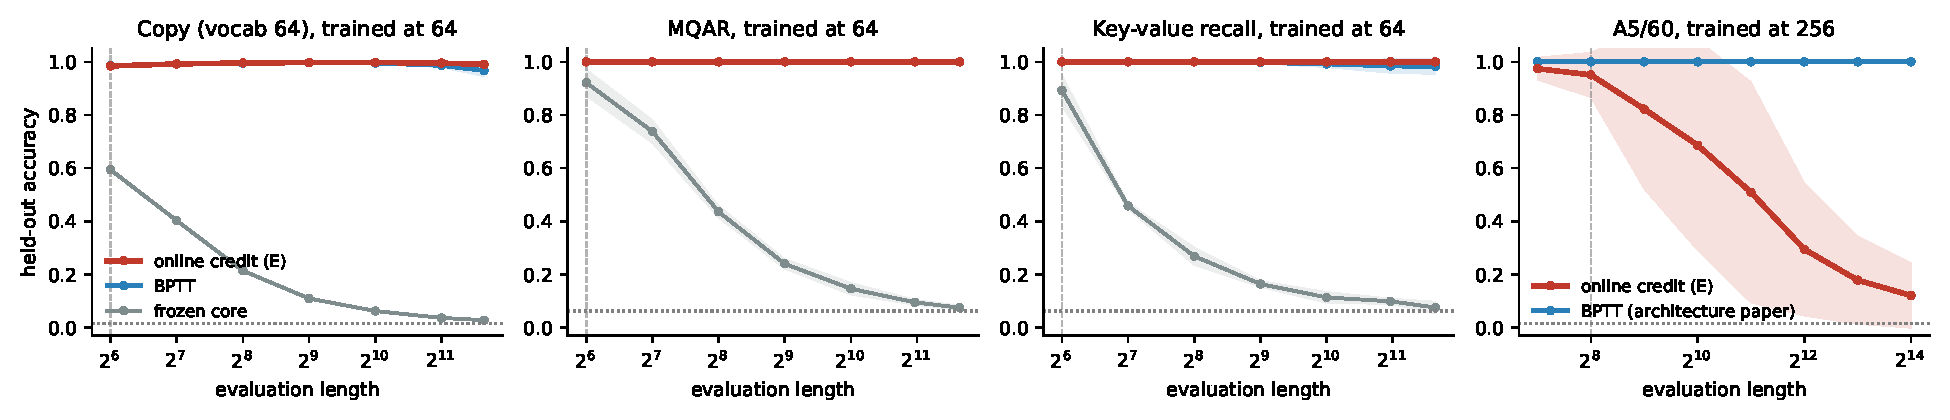
\includegraphics[width=\linewidth]{figs/fig1_continuity.pdf}
\caption{Continuity with the architecture experiments: held-out accuracy against
evaluation length (lines: seed means; bands: one standard deviation; dashed: training
length; dotted: chance). Copy, MQAR and key--value recall: three matched seeds of
online credit, BPTT and the frozen-core control. A5/60: the online cohort's held-out
seeds; BPTT is the architecture paper's two-seed result on the same model
\citep{rosdahl2026dabsn}.}
\label{fig:continuity}
\end{figure}

\begin{figure}[t]
\centering
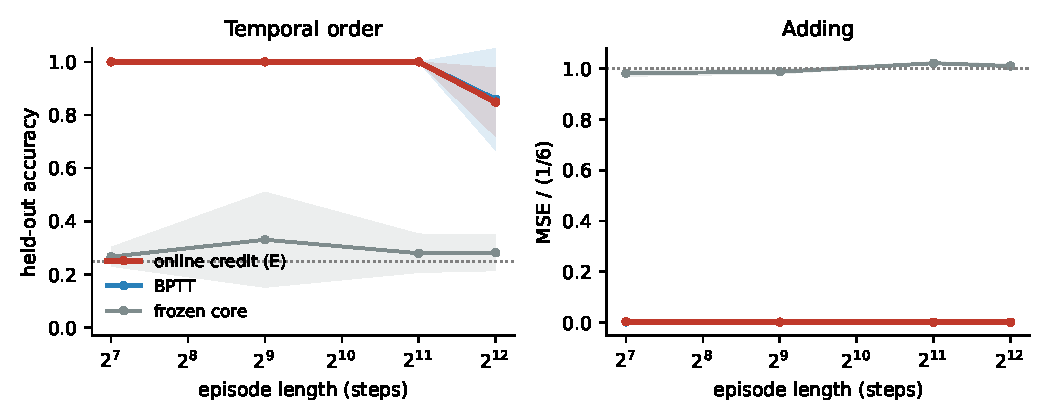
\includegraphics[width=0.8\linewidth]{figs/fig2_delayed.pdf}
\caption{The central study: final held-out performance against episode length for
online credit, BPTT and the frozen core (lines: seed means; bands: one standard
deviation). Temporal order: accuracy (dotted: chance, $1/4$). Adding: mean squared
error over $1/6$, the error of always predicting the mean sum (dotted).}
\label{fig:delayed}
\end{figure}

\begin{figure}[t]
\centering
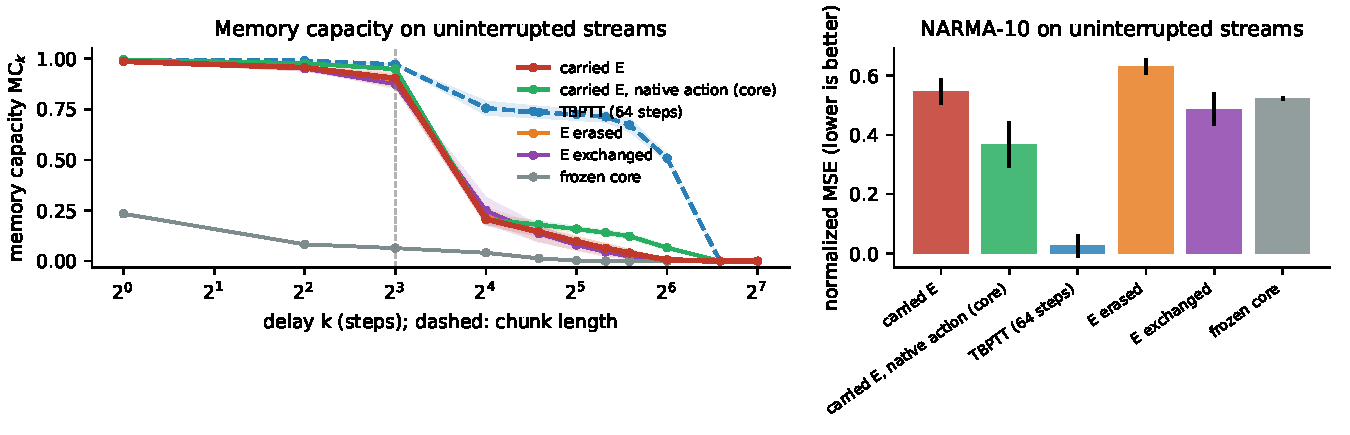
\includegraphics[width=\linewidth]{figs/fig3_streams.pdf}
\caption{Learning on uninterrupted streams, by arm. Left: memory capacity at each
delay (dashed: chunk length). Right: NARMA-10 normalized mean squared error.}
\label{fig:streams}
\end{figure}

\paragraph{Measured.}
\IfFileExists{results/generated.tex}{% Generated by reproduce/analysis.py from passed records. Do not edit.
All numbers below come from one results directory: device cuda, fp32 core compute, framework tree \texttt{680f9dd0e975}. Brackets are descriptive 95\% Student intervals over independent seeds.

\begin{table}[tbp]\centering\small\caption{Central delayed learning: final held-out score (accuracy for the temporal order problem, MSE over 1/6 for the adding problem).}
\begin{adjustbox}{max width=\linewidth}\begin{tabular}{llll}\toprule
task & length & method & mean [95\% CI] \\ \midrule
temporal order & 128 & online & 1.000 [1.000, 1.000] \\
temporal order & 128 & frozen core & 0.267 [0.222, 0.311] \\
temporal order & 128 & bptt & 1.000 [1.000, 1.000] \\
temporal order & 512 & online & 1.000 [1.000, 1.000] \\
temporal order & 512 & frozen core & 0.331 [0.108, 0.553] \\
temporal order & 512 & bptt & 1.000 [1.000, 1.000] \\
temporal order & 2048 & online & 1.000 [1.000, 1.000] \\
temporal order & 2048 & frozen core & 0.280 [0.190, 0.370] \\
temporal order & 2048 & bptt & 1.000 [1.000, 1.000] \\
temporal order & 4096 & online & 0.848 [0.688, 1.009] \\
temporal order & 4096 & frozen core & 0.282 [0.197, 0.366] \\
temporal order & 4096 & bptt & 0.859 [0.621, 1.097] \\
adding & 128 & online & 0.002 [$2.85\times10^{-4}$, 0.005] \\
adding & 128 & frozen core & 0.983 [0.967, 0.998] \\
adding & 128 & bptt & 0.002 [$7.68\times10^{-5}$, 0.005] \\
adding & 512 & online & 0.001 [$6.03\times10^{-4}$, 0.002] \\
adding & 512 & frozen core & 0.988 [0.978, 0.999] \\
adding & 512 & bptt & 0.001 [$-3.48\times10^{-4}$, 0.003] \\
adding & 2048 & online & $8.97\times10^{-4}$ [$5.41\times10^{-4}$, 0.001] \\
adding & 2048 & frozen core & 1.022 [1.014, 1.030] \\
adding & 2048 & bptt & 0.001 [$-5.67\times10^{-4}$, 0.003] \\
adding & 4096 & online & $9.28\times10^{-4}$ [$4.03\times10^{-4}$, 0.001] \\
adding & 4096 & frozen core & 1.011 [1.001, 1.021] \\
adding & 4096 & bptt & 0.001 [$-6.52\times10^{-4}$, 0.003] \\
\bottomrule\end{tabular}\end{adjustbox}\end{table}
\begin{table}[tbp]\centering\small\caption{Paired differences, online minus comparator (positive favors online).}
\begin{adjustbox}{max width=\linewidth}\begin{tabular}{llll}\toprule
task & length & comparison & mean [95\% CI] \\ \midrule
temporal order & 128 & online vs frozen core & 0.733 [0.689, 0.778] \\
temporal order & 128 & online vs bptt & 0.000 [0.000, 0.000] \\
temporal order & 512 & online vs frozen core & 0.669 [0.447, 0.892] \\
temporal order & 512 & online vs bptt & 0.000 [0.000, 0.000] \\
temporal order & 2048 & online vs frozen core & 0.720 [0.630, 0.810] \\
temporal order & 2048 & online vs bptt & 0.000 [0.000, 0.000] \\
temporal order & 4096 & online vs frozen core & 0.566 [0.441, 0.691] \\
temporal order & 4096 & online vs bptt & -0.011 [-0.188, 0.166] \\
adding & 128 & online vs frozen core & 0.980 [0.964, 0.997] \\
adding & 128 & online vs bptt & $-8.48\times10^{-5}$ [-0.003, 0.003] \\
adding & 512 & online vs frozen core & 0.987 [0.976, 0.998] \\
adding & 512 & online vs bptt & $2.04\times10^{-4}$ [-0.002, 0.002] \\
adding & 2048 & online vs frozen core & 1.021 [1.013, 1.029] \\
adding & 2048 & online vs bptt & $2.27\times10^{-4}$ [-0.002, 0.002] \\
adding & 4096 & online vs frozen core & 1.010 [1.000, 1.020] \\
adding & 4096 & online vs bptt & $2.05\times10^{-4}$ [-0.002, 0.002] \\
\bottomrule\end{tabular}\end{adjustbox}\end{table}
\begin{table}[tbp]\centering\small\caption{Shapes: final held-out score of online credit and BPTT at $(I,S)=(64,512)$ and $(128,256)$, one chunk per episode (accuracy for the temporal order problem, MSE over 1/6 for the adding problem; paired advantage positive favors online).}
\begin{adjustbox}{max width=\linewidth}\begin{tabular}{lllll}\toprule
task & $(I,S)$ & length & method & mean [95\% CI] \\ \midrule
temporal order & (64,512) & 128 & online & 1.000 [1.000, 1.000] \\
temporal order & (64,512) & 128 & bptt & 1.000 [1.000, 1.000] \\
temporal order & (64,512) & 128 & online minus bptt & 0.000 [0.000, 0.000] \\
temporal order & (64,512) & 512 & online & 1.000 [1.000, 1.000] \\
temporal order & (64,512) & 512 & bptt & 1.000 [1.000, 1.000] \\
temporal order & (64,512) & 512 & online minus bptt & 0.000 [0.000, 0.000] \\
temporal order & (64,512) & 2048 & online & 1.000 [1.000, 1.000] \\
temporal order & (64,512) & 2048 & bptt & 1.000 [1.000, 1.000] \\
temporal order & (64,512) & 2048 & online minus bptt & 0.000 [0.000, 0.000] \\
temporal order & (64,512) & 4096 & online & 0.725 [0.263, 1.186] \\
temporal order & (64,512) & 4096 & bptt & 0.937 [0.667, 1.207] \\
temporal order & (64,512) & 4096 & online minus bptt & -0.213 [-0.840, 0.415] \\
temporal order & (128,256) & 128 & online & 1.000 [1.000, 1.000] \\
temporal order & (128,256) & 128 & bptt & 1.000 [1.000, 1.000] \\
temporal order & (128,256) & 128 & online minus bptt & 0.000 [0.000, 0.000] \\
temporal order & (128,256) & 512 & online & 1.000 [1.000, 1.000] \\
temporal order & (128,256) & 512 & bptt & 1.000 [1.000, 1.000] \\
temporal order & (128,256) & 512 & online minus bptt & 0.000 [0.000, 0.000] \\
temporal order & (128,256) & 2048 & online & 1.000 [1.000, 1.000] \\
temporal order & (128,256) & 2048 & bptt & 1.000 [1.000, 1.000] \\
temporal order & (128,256) & 2048 & online minus bptt & 0.000 [0.000, 0.000] \\
temporal order & (128,256) & 4096 & online & 0.903 [0.600, 1.206] \\
temporal order & (128,256) & 4096 & bptt & 0.859 [0.396, 1.322] \\
temporal order & (128,256) & 4096 & online minus bptt & 0.044 [-0.535, 0.624] \\
adding & (64,512) & 128 & online & 0.004 [-0.002, 0.009] \\
adding & (64,512) & 128 & bptt & 0.003 [-0.003, 0.009] \\
adding & (64,512) & 128 & online minus bptt & $-8.65\times10^{-4}$ [-0.003, 0.002] \\
adding & (64,512) & 512 & online & 0.002 [$-1.29\times10^{-4}$, 0.005] \\
adding & (64,512) & 512 & bptt & 0.002 [-0.002, 0.006] \\
adding & (64,512) & 512 & online minus bptt & $-1.24\times10^{-4}$ [-0.002, 0.002] \\
adding & (64,512) & 2048 & online & 0.002 [$4.89\times10^{-4}$, 0.003] \\
adding & (64,512) & 2048 & bptt & 0.002 [-0.002, 0.006] \\
adding & (64,512) & 2048 & online minus bptt & $9.83\times10^{-5}$ [-0.003, 0.003] \\
adding & (64,512) & 4096 & online & 0.002 [$3.69\times10^{-4}$, 0.003] \\
adding & (64,512) & 4096 & bptt & 0.002 [-0.002, 0.005] \\
adding & (64,512) & 4096 & online minus bptt & $2.90\times10^{-5}$ [-0.002, 0.002] \\
adding & (128,256) & 128 & online & 0.004 [$-2.34\times10^{-4}$, 0.009] \\
adding & (128,256) & 128 & bptt & 0.002 [$1.78\times10^{-4}$, 0.003] \\
adding & (128,256) & 128 & online minus bptt & -0.003 [-0.008, 0.003] \\
adding & (128,256) & 512 & online & 0.003 [$8.61\times10^{-4}$, 0.004] \\
adding & (128,256) & 512 & bptt & 0.001 [$-7.35\times10^{-5}$, 0.002] \\
adding & (128,256) & 512 & online minus bptt & -0.001 [-0.003, $8.96\times10^{-5}$] \\
adding & (128,256) & 2048 & online & 0.002 [$7.80\times10^{-4}$, 0.003] \\
adding & (128,256) & 2048 & bptt & $9.95\times10^{-4}$ [$-1.32\times10^{-4}$, 0.002] \\
adding & (128,256) & 2048 & online minus bptt & -0.001 [-0.002, $-6.11\times10^{-4}$] \\
adding & (128,256) & 4096 & online & 0.002 [$-4.48\times10^{-4}$, 0.005] \\
adding & (128,256) & 4096 & bptt & $9.97\times10^{-4}$ [$-1.44\times10^{-4}$, 0.002] \\
adding & (128,256) & 4096 & online minus bptt & -0.001 [-0.003, $8.14\times10^{-4}$] \\
\bottomrule\end{tabular}\end{adjustbox}\end{table}
\begin{table}[tbp]\centering\small\caption{Frozen-checkpoint edits of $E$ at a boundary 1 or 32 steps before the query, against the carried branch: the core's credit (cosine and norm ratio) and held-out loss after one true update (positive favors carry); seeds averaged over evaluation lengths.}
\begin{adjustbox}{max width=\linewidth}\begin{tabular}{lllllll}\toprule
task & boundary & update & edit & credit cosine & credit norm ratio & post-update loss $-$ carry \\ \midrule
temporal order & 1 & 0 & zero & 0.118 [0.118, 0.118] & 0.118 [0.118, 0.118] & -0.011 [-0.012, -0.009] \\
temporal order & 1 & 0 & permute lanes & 0.999 [0.999, 1.000] & 1.000 [1.000, 1.000] & $1.45\times10^{-5}$ [$-6.46\times10^{-5}$, $9.36\times10^{-5}$] \\
temporal order & 1 & 0 & negate w & 1.000 [1.000, 1.000] & 1.000 [1.000, 1.000] & $-1.57\times10^{-5}$ [$-2.81\times10^{-5}$, $-3.28\times10^{-6}$] \\
temporal order & 1 & 0 & erase local & 0.121 [0.119, 0.123] & 0.121 [0.119, 0.123] & -0.010 [-0.011, -0.009] \\
temporal order & 1 & 1500 & zero & 0.435 [0.203, 0.668] & 0.232 [0.111, 0.354] & $9.82\times10^{-4}$ [-0.004, 0.006] \\
temporal order & 1 & 1500 & permute lanes & 0.999 [0.997, 1.000] & 1.001 [0.999, 1.003] & $-2.46\times10^{-5}$ [$-6.97\times10^{-5}$, $2.05\times10^{-5}$] \\
temporal order & 1 & 1500 & negate w & 1.000 [1.000, 1.000] & 1.000 [1.000, 1.000] & $6.57\times10^{-6}$ [$-8.96\times10^{-5}$, $1.03\times10^{-4}$] \\
temporal order & 1 & 1500 & erase local & 0.432 [0.241, 0.623] & 0.374 [0.274, 0.475] & $-4.18\times10^{-5}$ [$-5.48\times10^{-4}$, $4.64\times10^{-4}$] \\
temporal order & 1 & 4500 & zero & 0.507 [0.361, 0.653] & 0.231 [0.167, 0.295] & $6.10\times10^{-9}$ [$-7.58\times10^{-9}$, $1.98\times10^{-8}$] \\
temporal order & 1 & 4500 & permute lanes & 0.995 [0.985, 1.005] & 0.996 [0.985, 1.007] & $3.88\times10^{-11}$ [$-1.13\times10^{-10}$, $1.91\times10^{-10}$] \\
temporal order & 1 & 4500 & negate w & 1.000 [1.000, 1.000] & 1.000 [1.000, 1.000] & $3.10\times10^{-11}$ [$-3.17\times10^{-11}$, $9.38\times10^{-11}$] \\
temporal order & 1 & 4500 & erase local & 0.533 [0.410, 0.656] & 0.390 [0.336, 0.443] & $3.66\times10^{-9}$ [$-3.65\times10^{-9}$, $1.10\times10^{-8}$] \\
temporal order & 32 & 0 & zero & 1.000 [1.000, 1.000] & 0.981 [0.981, 0.981] & $-7.65\times10^{-6}$ [$-1.01\times10^{-5}$, $-5.16\times10^{-6}$] \\
temporal order & 32 & 0 & permute lanes & 1.000 [1.000, 1.000] & 1.000 [1.000, 1.000] & $-7.82\times10^{-8}$ [$-1.18\times10^{-6}$, $1.03\times10^{-6}$] \\
temporal order & 32 & 0 & negate w & 1.000 [1.000, 1.000] & 1.000 [1.000, 1.000] & $-3.26\times10^{-7}$ [$-7.78\times10^{-7}$, $1.27\times10^{-7}$] \\
temporal order & 32 & 0 & erase local & 1.000 [1.000, 1.000] & 0.981 [0.981, 0.981] & $-2.10\times10^{-7}$ [$-3.10\times10^{-7}$, $-1.09\times10^{-7}$] \\
temporal order & 32 & 1500 & zero & 0.999 [0.998, 1.000] & 0.984 [0.961, 1.008] & $8.51\times10^{-5}$ [$-2.12\times10^{-4}$, $3.82\times10^{-4}$] \\
temporal order & 32 & 1500 & permute lanes & 1.000 [1.000, 1.000] & 1.000 [1.000, 1.000] & $3.20\times10^{-7}$ [$-3.37\times10^{-7}$, $9.77\times10^{-7}$] \\
temporal order & 32 & 1500 & negate w & 1.000 [1.000, 1.000] & 1.000 [1.000, 1.000] & $-3.76\times10^{-8}$ [$-3.16\times10^{-7}$, $2.41\times10^{-7}$] \\
temporal order & 32 & 1500 & erase local & 0.999 [0.997, 1.000] & 0.987 [0.969, 1.005] & $8.40\times10^{-5}$ [$-1.98\times10^{-4}$, $3.66\times10^{-4}$] \\
temporal order & 32 & 4500 & zero & 0.986 [0.958, 1.014] & 0.963 [0.918, 1.008] & $4.73\times10^{-10}$ [$-8.67\times10^{-10}$, $1.81\times10^{-9}$] \\
temporal order & 32 & 4500 & permute lanes & 0.996 [0.987, 1.006] & 0.995 [0.982, 1.008] & $-3.10\times10^{-11}$ [$-9.38\times10^{-11}$, $3.17\times10^{-11}$] \\
temporal order & 32 & 4500 & negate w & 1.000 [1.000, 1.000] & 1.000 [1.000, 1.000] & 0.000 [0.000, 0.000] \\
temporal order & 32 & 4500 & erase local & 0.986 [0.958, 1.015] & 0.965 [0.923, 1.008] & $2.40\times10^{-10}$ [$-3.74\times10^{-10}$, $8.55\times10^{-10}$] \\
adding & 1 & 0 & zero & 0.059 [0.059, 0.060] & 0.060 [0.059, 0.060] & 0.153 [0.140, 0.166] \\
adding & 1 & 0 & permute lanes & 1.000 [1.000, 1.000] & 1.000 [1.000, 1.000] & $-1.41\times10^{-6}$ [$-7.49\times10^{-6}$, $4.67\times10^{-6}$] \\
adding & 1 & 0 & negate w & 1.000 [1.000, 1.000] & 1.000 [1.000, 1.000] & $6.62\times10^{-6}$ [$-1.03\times10^{-5}$, $2.36\times10^{-5}$] \\
adding & 1 & 0 & erase local & 0.061 [0.060, 0.061] & 0.061 [0.060, 0.062] & 0.129 [0.118, 0.140] \\
adding & 1 & 1500 & zero & 0.342 [0.013, 0.671] & 0.132 [0.091, 0.173] & $-7.93\times10^{-5}$ [$-1.98\times10^{-4}$, $3.94\times10^{-5}$] \\
adding & 1 & 1500 & permute lanes & 1.000 [1.000, 1.000] & 1.000 [1.000, 1.000] & $3.36\times10^{-7}$ [$-2.24\times10^{-7}$, $8.97\times10^{-7}$] \\
adding & 1 & 1500 & negate w & 1.000 [1.000, 1.000] & 1.000 [1.000, 1.000] & $8.33\times10^{-8}$ [$-1.11\times10^{-7}$, $2.78\times10^{-7}$] \\
adding & 1 & 1500 & erase local & 0.341 [0.172, 0.510] & 0.187 [0.166, 0.207] & $-4.59\times10^{-6}$ [$-8.46\times10^{-5}$, $7.54\times10^{-5}$] \\
adding & 1 & 4500 & zero & 0.300 [0.040, 0.559] & 0.146 [0.099, 0.194] & $-1.64\times10^{-5}$ [$-5.57\times10^{-5}$, $2.29\times10^{-5}$] \\
adding & 1 & 4500 & permute lanes & 1.000 [0.999, 1.000] & 1.000 [1.000, 1.000] & $2.64\times10^{-8}$ [$-1.42\times10^{-7}$, $1.94\times10^{-7}$] \\
adding & 1 & 4500 & negate w & 1.000 [1.000, 1.000] & 1.000 [1.000, 1.000] & $2.57\times10^{-8}$ [$-4.93\times10^{-8}$, $1.01\times10^{-7}$] \\
adding & 1 & 4500 & erase local & 0.321 [0.149, 0.494] & 0.172 [0.139, 0.204] & $-1.52\times10^{-5}$ [$-5.05\times10^{-5}$, $2.01\times10^{-5}$] \\
adding & 32 & 0 & zero & 1.000 [1.000, 1.000] & 0.981 [0.980, 0.981] & $3.44\times10^{-6}$ [$-5.35\times10^{-6}$, $1.22\times10^{-5}$] \\
adding & 32 & 0 & permute lanes & 1.000 [1.000, 1.000] & 1.000 [1.000, 1.000] & $4.38\times10^{-8}$ [$-1.35\times10^{-7}$, $2.22\times10^{-7}$] \\
adding & 32 & 0 & negate w & 1.000 [1.000, 1.000] & 1.000 [1.000, 1.000] & $5.89\times10^{-8}$ [$-2.45\times10^{-7}$, $3.62\times10^{-7}$] \\
adding & 32 & 0 & erase local & 1.000 [1.000, 1.000] & 0.981 [0.980, 0.981] & $-1.64\times10^{-7}$ [$-2.65\times10^{-7}$, $-6.33\times10^{-8}$] \\
adding & 32 & 1500 & zero & 0.983 [0.972, 0.994] & 0.929 [0.907, 0.951] & $3.10\times10^{-5}$ [$-1.20\times10^{-5}$, $7.40\times10^{-5}$] \\
adding & 32 & 1500 & permute lanes & 1.000 [1.000, 1.000] & 1.000 [1.000, 1.000] & $1.14\times10^{-6}$ [$-2.41\times10^{-7}$, $2.51\times10^{-6}$] \\
adding & 32 & 1500 & negate w & 1.000 [1.000, 1.000] & 1.000 [1.000, 1.000] & $-1.51\times10^{-8}$ [$-3.32\times10^{-8}$, $2.94\times10^{-9}$] \\
adding & 32 & 1500 & erase local & 0.983 [0.972, 0.994] & 0.929 [0.908, 0.951] & $3.10\times10^{-5}$ [$-1.41\times10^{-5}$, $7.61\times10^{-5}$] \\
adding & 32 & 4500 & zero & 0.976 [0.967, 0.985] & 0.946 [0.933, 0.960] & $8.09\times10^{-7}$ [$-3.64\times10^{-6}$, $5.25\times10^{-6}$] \\
adding & 32 & 4500 & permute lanes & 1.000 [1.000, 1.000] & 1.000 [1.000, 1.000] & $-1.77\times10^{-8}$ [$-8.30\times10^{-8}$, $4.75\times10^{-8}$] \\
adding & 32 & 4500 & negate w & 1.000 [1.000, 1.000] & 1.000 [1.000, 1.000] & $-6.40\times10^{-10}$ [$-3.44\times10^{-9}$, $2.16\times10^{-9}$] \\
adding & 32 & 4500 & erase local & 0.976 [0.967, 0.985] & 0.946 [0.933, 0.960] & $8.23\times10^{-7}$ [$-3.49\times10^{-6}$, $5.14\times10^{-6}$] \\
\bottomrule\end{tabular}\end{adjustbox}\end{table}
\begin{table}[tbp]\centering\small\caption{Erased isolated historical pathway at the checkpoint (1-step boundary, final input zeroed): $W$'s credit is purely historical.}
\begin{adjustbox}{max width=\linewidth}\begin{tabular}{llll}\toprule
task & update & cosine, negated $W$ trace to carry & norm ratio, erased $E$ to carry \\ \midrule
temporal order & 0 & -1.000 [-1.000, -1.000] & 0.000 [0.000, 0.000] \\
temporal order & 1500 & -1.000 [-1.000, -1.000] & 0.000 [0.000, 0.000] \\
temporal order & 4500 & -1.000 [-1.000, -1.000] & 0.000 [0.000, 0.000] \\
adding & 0 & -1.000 [-1.000, -1.000] & 0.000 [0.000, 0.000] \\
adding & 1500 & -1.000 [-1.000, -1.000] & 0.000 [0.000, 0.000] \\
adding & 4500 & -1.000 [-1.000, -1.000] & 0.000 [0.000, 0.000] \\
\bottomrule\end{tabular}\end{adjustbox}\end{table}
\begin{table}[tbp]\centering\small\caption{Memory capacity on uninterrupted streams (stock core, no read). Mean [95\% CI] by arm.}
\begin{adjustbox}{max width=\linewidth}\begin{tabular}{llllll}\toprule
metric & carry & reset & permute & frozen core & tbptt \\ \midrule
memory capacity total & 3.405 [3.219, 3.592] & 3.382 [3.157, 3.606] & 3.348 [3.189, 3.508] & 0.439 [0.430, 0.449] & 7.065 [6.852, 7.279] \\
memory capacity delay 1 & 0.987 [0.982, 0.992] & 0.986 [0.981, 0.992] & 0.986 [0.981, 0.992] & 0.234 [0.232, 0.235] & 0.994 [0.994, 0.995] \\
memory capacity delay 4 & 0.956 [0.933, 0.978] & 0.957 [0.947, 0.966] & 0.951 [0.938, 0.964] & 0.083 [0.080, 0.086] & 0.990 [0.989, 0.992] \\
memory capacity delay 8 & 0.903 [0.866, 0.940] & 0.887 [0.842, 0.932] & 0.874 [0.855, 0.892] & 0.064 [0.062, 0.067] & 0.972 [0.968, 0.976] \\
memory capacity delay 16 & 0.207 [0.169, 0.246] & 0.230 [0.186, 0.273] & 0.250 [0.169, 0.331] & 0.041 [0.038, 0.044] & 0.756 [0.713, 0.799] \\
memory capacity delay 24 & 0.145 [0.117, 0.173] & 0.140 [0.089, 0.192] & 0.137 [0.084, 0.190] & 0.014 [0.012, 0.016] & 0.735 [0.699, 0.772] \\
memory capacity delay 32 & 0.097 [0.069, 0.124] & 0.089 [0.044, 0.134] & 0.080 [0.050, 0.109] & 0.003 [0.002, 0.003] & 0.724 [0.688, 0.759] \\
memory capacity delay 40 & 0.064 [0.033, 0.094] & 0.054 [0.015, 0.093] & 0.045 [0.025, 0.065] & $1.48\times10^{-4}$ [$8.32\times10^{-5}$, $2.12\times10^{-4}$] & 0.713 [0.680, 0.745] \\
memory capacity delay 48 & 0.040 [0.018, 0.062] & 0.035 [0.006, 0.064] & 0.023 [0.011, 0.034] & $3.14\times10^{-6}$ [$-2.03\times10^{-6}$, $8.30\times10^{-6}$] & 0.672 [0.632, 0.712] \\
memory capacity delay 64 & 0.006 [0.004, 0.008] & 0.004 [0.002, 0.007] & 0.003 [$9.10\times10^{-4}$, 0.005] & $2.14\times10^{-5}$ [$-1.97\times10^{-5}$, $6.26\times10^{-5}$] & 0.509 [0.487, 0.531] \\
memory capacity delay 96 & $4.54\times10^{-4}$ [$2.04\times10^{-4}$, $7.04\times10^{-4}$] & $1.87\times10^{-4}$ [$-2.68\times10^{-5}$, $4.01\times10^{-4}$] & $1.26\times10^{-4}$ [$5.76\times10^{-6}$, $2.46\times10^{-4}$] & $1.52\times10^{-5}$ [$-1.50\times10^{-5}$, $4.54\times10^{-5}$] & $7.05\times10^{-5}$ [$-1.45\times10^{-5}$, $1.55\times10^{-4}$] \\
memory capacity delay 128 & $7.43\times10^{-5}$ [$-4.69\times10^{-5}$, $1.96\times10^{-4}$] & $2.37\times10^{-5}$ [$4.54\times10^{-6}$, $4.29\times10^{-5}$] & $2.22\times10^{-5}$ [$7.75\times10^{-6}$, $3.66\times10^{-5}$] & $2.40\times10^{-5}$ [$8.98\times10^{-6}$, $3.90\times10^{-5}$] & $8.20\times10^{-6}$ [$-5.88\times10^{-6}$, $2.23\times10^{-5}$] \\
\bottomrule\end{tabular}\end{adjustbox}\end{table}
\begin{table}[tbp]\centering\small\caption{Memory capacity on uninterrupted streams: per-unit bound of carried $E$ and the transport diagnostic at final weights (log-growth per step; Jacobian rate $<0$: full dynamics contract).}
\begin{adjustbox}{max width=\linewidth}\begin{tabular}{lllllll}\toprule
arm & seed & rescalings & units & expanding units & fastest unit rate & Jacobian rate \\ \midrule
carry & 100 & 130 & 2 & 2 & 0.0022 & -0.0028 \\
carry & 101 & 4 & 1 & 0 & $7.729\times10^{-4}$ & -0.0072 \\
carry & 102 & 6 & 2 & 0 & $7.128\times10^{-4}$ & -0.0013 \\
carry & 103 & 0 & 0 & 2 & 0.0044 & -0.0021 \\
carry & 104 & 0 & 0 & 0 & $8.730\times10^{-4}$ & -0.0056 \\
\bottomrule\end{tabular}\end{adjustbox}\end{table}
\begin{table}[tbp]\centering\small\caption{Memory capacity on uninterrupted streams: paired contrasts (positive favors carried $E$).}
\begin{adjustbox}{max width=\linewidth}\begin{tabular}{ll}\toprule
contrast & mean [95\% CI] \\ \midrule
carry versus reset & 0.024 [-0.244, 0.292] \\
carry versus permute & 0.057 [-0.083, 0.197] \\
carry versus frozen core & 2.966 [2.777, 3.155] \\
carry versus tbptt & -3.660 [-3.983, -3.336] \\
\bottomrule\end{tabular}\end{adjustbox}\end{table}
\begin{table}[tbp]\centering\small\caption{NARMA-10 on uninterrupted streams (stock core, no read): normalized MSE. Mean [95\% CI] by arm.}
\begin{adjustbox}{max width=\linewidth}\begin{tabular}{llllll}\toprule
metric & carry & reset & permute & frozen core & tbptt \\ \midrule
nmse & 0.545 [0.490, 0.601] & 0.630 [0.597, 0.664] & 0.486 [0.418, 0.555] & 0.523 [0.516, 0.530] & 0.026 [-0.022, 0.073] \\
\bottomrule\end{tabular}\end{adjustbox}\end{table}
\begin{table}[tbp]\centering\small\caption{NARMA-10 on uninterrupted streams: per-unit bound of carried $E$ and the transport diagnostic at final weights (log-growth per step; Jacobian rate $<0$: full dynamics contract).}
\begin{adjustbox}{max width=\linewidth}\begin{tabular}{lllllll}\toprule
arm & seed & rescalings & units & expanding units & fastest unit rate & Jacobian rate \\ \midrule
carry & 100 & 101 & 1 & 0 & $7.977\times10^{-4}$ & -0.0034 \\
carry & 101 & 0 & 0 & 0 & $6.880\times10^{-4}$ & 0.0126 \\
carry & 102 & 398 & 5 & 3 & 0.0011 & 0.0133 \\
carry & 103 & 139 & 6 & 1 & 0.0012 & 0.0048 \\
carry & 104 & 701 & 2 & 2 & 0.0254 & 0.0154 \\
\bottomrule\end{tabular}\end{adjustbox}\end{table}
\begin{table}[tbp]\centering\small\caption{NARMA-10 on uninterrupted streams: paired contrasts (positive favors carried $E$).}
\begin{adjustbox}{max width=\linewidth}\begin{tabular}{ll}\toprule
contrast & mean [95\% CI] \\ \midrule
carry versus reset & 0.085 [0.013, 0.157] \\
carry versus permute & -0.059 [-0.153, 0.035] \\
carry versus frozen core & -0.022 [-0.076, 0.031] \\
carry versus tbptt & -0.520 [-0.573, -0.467] \\
\bottomrule\end{tabular}\end{adjustbox}\end{table}
\begin{table}[tbp]\centering\small\caption{The conjunction: learning driven entirely by $E$ (native) against AdamW with online credit and with BPTT; held-out accuracy by evaluation length, mean [95\% CI] by arm.}
\begin{adjustbox}{max width=\linewidth}\begin{tabular}{lllllll}\toprule
task & length & native & adamw online & adamw bptt & native minus adamw online & native minus adamw bptt \\ \midrule
copy & 64 & 0.994 [0.973, 1.016] & 0.985 [0.984, 0.985] & 0.986 [0.982, 0.990] & 0.010 [-0.012, 0.031] & 0.009 [-0.011, 0.028] \\
copy & 128 & 0.997 [0.987, 1.007] & 0.992 [0.992, 0.992] & 0.992 [0.992, 0.993] & 0.005 [-0.006, 0.015] & 0.005 [-0.005, 0.014] \\
copy & 256 & 0.998 [0.993, 1.002] & 0.996 [0.996, 0.996] & 0.996 [0.995, 0.996] & 0.002 [-0.002, 0.006] & 0.002 [-0.002, 0.007] \\
copy & 512 & 0.998 [0.996, 1.000] & 0.997 [0.997, 0.998] & 0.997 [0.996, 0.998] & $5.05\times10^{-4}$ [-0.001, 0.002] & 0.001 [-0.002, 0.004] \\
copy & 1024 & 0.997 [0.995, 0.999] & 0.998 [0.997, 0.999] & 0.996 [0.992, 1.000] & $-8.02\times10^{-4}$ [-0.004, 0.002] & $9.52\times10^{-4}$ [-0.001, 0.003] \\
copy & 2048 & 0.991 [0.984, 0.999] & 0.995 [0.994, 0.997] & 0.987 [0.965, 1.008] & -0.004 [-0.013, 0.005] & 0.005 [-0.010, 0.019] \\
copy & 3200 & 0.983 [0.964, 1.001] & 0.990 [0.986, 0.995] & 0.967 [0.912, 1.023] & -0.008 [-0.030, 0.015] & 0.015 [-0.024, 0.055] \\
mqar & 64 & 1.000 [1.000, 1.000] & 1.000 [1.000, 1.000] & 1.000 [1.000, 1.000] & 0.000 [0.000, 0.000] & 0.000 [0.000, 0.000] \\
mqar & 128 & 1.000 [1.000, 1.000] & 1.000 [1.000, 1.000] & 1.000 [1.000, 1.000] & 0.000 [0.000, 0.000] & 0.000 [0.000, 0.000] \\
mqar & 256 & 1.000 [1.000, 1.000] & 1.000 [1.000, 1.000] & 1.000 [1.000, 1.000] & $-6.51\times10^{-5}$ [$-3.45\times10^{-4}$, $2.15\times10^{-4}$] & $-6.51\times10^{-5}$ [$-3.45\times10^{-4}$, $2.15\times10^{-4}$] \\
mqar & 512 & 1.000 [1.000, 1.000] & 1.000 [1.000, 1.000] & 1.000 [1.000, 1.000] & $-6.51\times10^{-5}$ [$-3.45\times10^{-4}$, $2.15\times10^{-4}$] & $-6.51\times10^{-5}$ [$-3.45\times10^{-4}$, $2.15\times10^{-4}$] \\
mqar & 1024 & 1.000 [1.000, 1.000] & 1.000 [1.000, 1.000] & 1.000 [1.000, 1.000] & $-1.30\times10^{-4}$ [$-4.10\times10^{-4}$, $1.50\times10^{-4}$] & $-1.30\times10^{-4}$ [$-4.10\times10^{-4}$, $1.50\times10^{-4}$] \\
mqar & 2000 & 1.000 [1.000, 1.000] & 1.000 [1.000, 1.000] & 1.000 [1.000, 1.000] & $-6.51\times10^{-5}$ [$-3.45\times10^{-4}$, $2.15\times10^{-4}$] & $-6.51\times10^{-5}$ [$-3.45\times10^{-4}$, $2.15\times10^{-4}$] \\
mqar & 3200 & 1.000 [1.000, 1.000] & 1.000 [1.000, 1.000] & 1.000 [1.000, 1.000] & 0.000 [0.000, 0.000] & 0.000 [0.000, 0.000] \\
keyvalue & 64 & 0.999 [0.994, 1.003] & 1.000 [1.000, 1.000] & 1.000 [1.000, 1.000] & -0.001 [-0.006, 0.003] & -0.001 [-0.006, 0.003] \\
keyvalue & 128 & 0.999 [0.997, 1.002] & 1.000 [1.000, 1.000] & 1.000 [1.000, 1.000] & $-5.21\times10^{-4}$ [-0.003, 0.002] & $-5.21\times10^{-4}$ [-0.003, 0.002] \\
keyvalue & 256 & 1.000 [1.000, 1.000] & 1.000 [1.000, 1.000] & 1.000 [1.000, 1.000] & 0.000 [0.000, 0.000] & 0.000 [0.000, 0.000] \\
keyvalue & 512 & 0.999 [0.997, 1.002] & 1.000 [1.000, 1.000] & 0.997 [0.986, 1.009] & $-5.21\times10^{-4}$ [-0.003, 0.002] & 0.002 [-0.010, 0.015] \\
keyvalue & 1024 & 1.000 [1.000, 1.000] & 1.000 [1.000, 1.000] & 0.992 [0.959, 1.026] & 0.000 [0.000, 0.000] & 0.008 [-0.026, 0.041] \\
keyvalue & 2000 & 1.000 [1.000, 1.000] & 1.000 [1.000, 1.000] & 0.984 [0.917, 1.052] & 0.000 [0.000, 0.000] & 0.016 [-0.052, 0.083] \\
keyvalue & 3200 & 0.999 [0.997, 1.002] & 1.000 [1.000, 1.000] & 0.983 [0.909, 1.057] & $-5.21\times10^{-4}$ [-0.003, 0.002] & 0.017 [-0.058, 0.092] \\
\bottomrule\end{tabular}\end{adjustbox}\end{table}
\begin{table}[tbp]\centering\small\caption{Data efficiency: first scheduled update reaching 0.99 held-out accuracy at the training length (-- never).}
\begin{adjustbox}{max width=\linewidth}\begin{tabular}{llll}\toprule
task & arm & seed & update \\ \midrule
copy & native & 0 & 400 \\
copy & native & 1 & 400 \\
copy & native & 2 & -- \\
copy & adamw online & 0 & -- \\
copy & adamw online & 1 & -- \\
copy & adamw online & 2 & -- \\
copy & adamw bptt & 0 & -- \\
copy & adamw bptt & 1 & -- \\
copy & adamw bptt & 2 & -- \\
mqar & native & 0 & 200 \\
mqar & native & 1 & 200 \\
mqar & native & 2 & 200 \\
mqar & adamw online & 0 & 300 \\
mqar & adamw online & 1 & 200 \\
mqar & adamw online & 2 & 200 \\
mqar & adamw bptt & 0 & 200 \\
mqar & adamw bptt & 1 & 200 \\
mqar & adamw bptt & 2 & 200 \\
keyvalue & native & 0 & 500 \\
keyvalue & native & 1 & 700 \\
keyvalue & native & 2 & 500 \\
keyvalue & adamw online & 0 & 200 \\
keyvalue & adamw online & 1 & 500 \\
keyvalue & adamw online & 2 & 300 \\
keyvalue & adamw bptt & 0 & 300 \\
keyvalue & adamw bptt & 1 & 700 \\
keyvalue & adamw bptt & 2 & 200 \\
\bottomrule\end{tabular}\end{adjustbox}\end{table}
\begin{table}[tbp]\centering\small\caption{Moment-free normalized action on the stream benchmarks.}
\begin{adjustbox}{max width=\linewidth}\begin{tabular}{lll}\toprule
benchmark & arm & mean [95\% CI] \\ \midrule
continuous & carried E with Adam & 3.405 [3.219, 3.592] \\
continuous & native action on the core & 3.795 [3.707, 3.883] \\
continuous & native minus Adam (positive favors native) & 0.390 [0.171, 0.608] \\
sustained & carried E with Adam & 0.545 [0.490, 0.601] \\
sustained & native action on the core & 0.367 [0.270, 0.463] \\
sustained & native minus Adam (positive favors native) & 0.179 [0.048, 0.310] \\
\bottomrule\end{tabular}\end{adjustbox}\end{table}
\begin{table}[tbp]\centering\small\caption{Stream benchmarks at matched credit reach.}
\begin{adjustbox}{max width=\linewidth}\begin{tabular}{llll}\toprule
benchmark & reach & arm & mean [95\% CI] \\ \midrule
continuous & 1 chunk & exact BPTT & 4.467 [4.369, 4.565] \\
continuous & 1 chunk & erased E & 3.382 [3.157, 3.606] \\
continuous & 1 chunk & exact minus E (positive favors exact) & 1.085 [0.926, 1.245] \\
continuous & 8 chunks vs unbounded & exact BPTT minus carried E (positive favors exact) & 3.660 [3.336, 3.983] \\
sustained & 1 chunk & exact BPTT & 0.606 [0.578, 0.634] \\
sustained & 1 chunk & erased E & 0.630 [0.597, 0.664] \\
sustained & 1 chunk & exact minus E (positive favors exact) & 0.024 [-0.002, 0.051] \\
sustained & 8 chunks vs unbounded & exact BPTT minus carried E (positive favors exact) & 0.520 [0.467, 0.573] \\
\bottomrule\end{tabular}\end{adjustbox}\end{table}
\begin{table}[tbp]\centering\small\caption{Online versus exact credit at trained stream weights, by parameter family (windows of 64 steps).}
\begin{adjustbox}{max width=\linewidth}\begin{tabular}{llll}\toprule
benchmark & family & metric & mean [95\% CI] \\ \midrule
continuous & A & cosine & 0.301 [0.179, 0.423] \\
continuous & A & norm ratio online/exact & 0.517 [0.210, 0.825] \\
continuous & Ug & cosine & 0.309 [0.176, 0.442] \\
continuous & Ug & norm ratio online/exact & 0.393 [0.246, 0.541] \\
continuous & W & cosine & 0.247 [0.210, 0.284] \\
continuous & W & norm ratio online/exact & 0.180 [0.150, 0.209] \\
continuous & Wg & cosine & 0.318 [0.177, 0.458] \\
continuous & Wg & norm ratio online/exact & 0.351 [0.263, 0.440] \\
continuous & all & cosine & 0.318 [0.247, 0.389] \\
continuous & all & norm ratio online/exact & 0.466 [0.332, 0.600] \\
continuous & local controls & cosine & 0.289 [0.228, 0.350] \\
continuous & local controls & norm ratio online/exact & 0.512 [0.352, 0.672] \\
continuous & readout & cosine & 1.000 [1.000, 1.000] \\
continuous & readout & norm ratio online/exact & 1.000 [1.000, 1.000] \\
continuous & shared controls & cosine & 0.445 [0.081, 0.809] \\
continuous & shared controls & norm ratio online/exact & 0.390 [-0.105, 0.885] \\
sustained & A & cosine & 0.542 [0.282, 0.802] \\
sustained & A & norm ratio online/exact & 1.177 [-1.285, 3.640] \\
sustained & Ug & cosine & 0.450 [0.158, 0.742] \\
sustained & Ug & norm ratio online/exact & 0.566 [0.106, 1.026] \\
sustained & W & cosine & 0.389 [0.142, 0.637] \\
sustained & W & norm ratio online/exact & 0.434 [-0.285, 1.154] \\
sustained & Wg & cosine & 0.478 [0.172, 0.783] \\
sustained & Wg & norm ratio online/exact & 0.872 [-0.290, 2.035] \\
sustained & all & cosine & 0.421 [0.273, 0.568] \\
sustained & all & norm ratio online/exact & 0.829 [-0.353, 2.012] \\
sustained & local controls & cosine & 0.336 [0.178, 0.494] \\
sustained & local controls & norm ratio online/exact & 0.770 [-0.603, 2.142] \\
sustained & readout & cosine & 1.000 [1.000, 1.000] \\
sustained & readout & norm ratio online/exact & 1.000 [1.000, 1.000] \\
sustained & shared controls & cosine & 0.422 [-0.023, 0.866] \\
sustained & shared controls & norm ratio online/exact & 0.565 [-0.115, 1.245] \\
\bottomrule\end{tabular}\end{adjustbox}\end{table}
\begin{table}[tbp]\centering\small\caption{Continuity with paper 1: online minus BPTT accuracy.}
\begin{adjustbox}{max width=\linewidth}\begin{tabular}{llll}\toprule
task & length & mean [95\% CI] & no loss $>$ 2 pts supported \\ \midrule
copy & 64 & -0.001 [-0.005, 0.003] & yes \\
copy & 128 & $-1.95\times10^{-4}$ [-0.001, $8.15\times10^{-4}$] & yes \\
copy & 256 & $3.58\times10^{-4}$ [$-1.01\times10^{-4}$, $8.17\times10^{-4}$] & yes \\
copy & 512 & $5.05\times10^{-4}$ [-0.001, 0.002] & yes \\
copy & 1024 & 0.002 [-0.003, 0.007] & yes \\
copy & 2048 & 0.009 [-0.014, 0.032] & yes \\
copy & 3200 & 0.023 [-0.037, 0.083] & no \\
mqar & 64 & 0.000 [0.000, 0.000] & yes \\
mqar & 128 & 0.000 [0.000, 0.000] & yes \\
mqar & 256 & 0.000 [0.000, 0.000] & yes \\
mqar & 512 & 0.000 [0.000, 0.000] & yes \\
mqar & 1024 & 0.000 [0.000, 0.000] & yes \\
mqar & 2000 & 0.000 [0.000, 0.000] & yes \\
mqar & 3200 & 0.000 [0.000, 0.000] & yes \\
keyvalue & 64 & 0.000 [0.000, 0.000] & yes \\
keyvalue & 128 & 0.000 [0.000, 0.000] & yes \\
keyvalue & 256 & 0.000 [0.000, 0.000] & yes \\
keyvalue & 512 & 0.003 [-0.009, 0.014] & yes \\
keyvalue & 1024 & 0.008 [-0.026, 0.041] & no \\
keyvalue & 2000 & 0.016 [-0.052, 0.083] & no \\
keyvalue & 3200 & 0.017 [-0.057, 0.091] & no \\
\bottomrule\end{tabular}\end{adjustbox}\end{table}
\begin{table}[tbp]\centering\small\caption{A5/60 frozen-rate cohort (online).}
\begin{adjustbox}{max width=\linewidth}\begin{tabular}{lll}\toprule
seed & role & exact at every length \\ \midrule
0 & development & no \\
1 & heldout & no \\
2 & heldout & no \\
3 & heldout & no \\
\bottomrule\end{tabular}\end{adjustbox}\end{table}
\begin{table}[tbp]\centering\small\caption{A5/60 accuracy by evaluation length under online credit (trained at 256).}
\begin{adjustbox}{max width=\linewidth}\begin{tabular}{lll}\toprule
length & held-out seeds, mean [95\% CI] & development seed 0 \\ \midrule
128 & 0.974 [0.868, 1.080] & 1.000 \\
256 & 0.951 [0.739, 1.162] & 1.000 \\
512 & 0.822 [0.072, 1.572] & 1.000 \\
1024 & 0.686 [-0.298, 1.671] & 0.901 \\
2048 & 0.509 [-0.525, 1.543] & 0.532 \\
4096 & 0.295 [-0.329, 0.918] & 0.350 \\
8192 & 0.179 [-0.234, 0.591] & 0.258 \\
16384 & 0.121 [-0.184, 0.425] & 0.211 \\
\bottomrule\end{tabular}\end{adjustbox}\end{table}
\begin{table}[tbp]\centering\small\caption{Objective-conditioned continuation: last-half pre-action MSE.}
\begin{adjustbox}{max width=\linewidth}\begin{tabular}{ll}\toprule
control & mean [95\% CI] \\ \midrule
retained & 0.003 [0.002, 0.003] \\
erased & 0.033 [0.028, 0.038] \\
exchanged & 0.120 [0.099, 0.141] \\
k y erased & 0.033 [0.028, 0.038] \\
\bottomrule\end{tabular}\end{adjustbox}\end{table}
\begin{table}[tbp]\centering\small\caption{Held-out objective directions: last-half pre-action MSE.}
\begin{adjustbox}{max width=\linewidth}\begin{tabular}{ll}\toprule
control & mean [95\% CI] \\ \midrule
retained & 0.002 [0.001, 0.002] \\
erased & 0.017 [0.016, 0.019] \\
exchanged & 0.066 [0.060, 0.073] \\
k y erased & 0.017 [0.016, 0.019] \\
frozen reader & 0.001 [$9.45\times10^{-4}$, 0.001] \\
adaptive amplitude & 0.002 [0.001, 0.002] \\
\bottomrule\end{tabular}\end{adjustbox}\end{table}
\begin{table}[tbp]\centering\small\caption{Teacher matching by direct action: $\ell_2$ error reduction after each action.}
\begin{adjustbox}{max width=\linewidth}\begin{tabular}{llll}\toprule
perturbation & method & action & mean [95\% CI] \\ \midrule
0.001 & E inverse & 1 & 0.824 [0.791, 0.858] \\
0.001 & E inverse & 2 & 0.966 [0.953, 0.980] \\
0.001 & E inverse & 3 & 0.986 [0.975, 0.997] \\
0.001 & E inverse & 4 & 0.987 [0.975, 0.998] \\
0.001 & H inverse & 1 & 0.987 [0.975, 0.998] \\
0.001 & H inverse & 2 & 0.987 [0.975, 0.999] \\
0.001 & H inverse & 3 & 0.987 [0.975, 0.999] \\
0.001 & H inverse & 4 & 0.987 [0.975, 0.999] \\
0.001 & E adjoint matched norm & 1 & -0.138 [-1.393, 1.117] \\
0.001 & E adjoint matched norm & 2 & -0.067 [-1.247, 1.113] \\
0.001 & E adjoint matched norm & 3 & -0.325 [-2.158, 1.508] \\
0.001 & E adjoint matched norm & 4 & -0.172 [-1.363, 1.019] \\
0.001 & no action & 1 & 0.000 [0.000, 0.000] \\
0.001 & no action & 2 & 0.000 [0.000, 0.000] \\
0.001 & no action & 3 & 0.000 [0.000, 0.000] \\
0.001 & no action & 4 & 0.000 [0.000, 0.000] \\
0.01 & E inverse & 1 & 0.825 [0.791, 0.859] \\
0.01 & E inverse & 2 & 0.967 [0.953, 0.980] \\
0.01 & E inverse & 3 & 0.986 [0.975, 0.997] \\
0.01 & E inverse & 4 & 0.987 [0.976, 0.998] \\
0.01 & H inverse & 1 & 0.986 [0.975, 0.997] \\
0.01 & H inverse & 2 & 0.987 [0.976, 0.998] \\
0.01 & H inverse & 3 & 0.987 [0.976, 0.998] \\
0.01 & H inverse & 4 & 0.987 [0.976, 0.998] \\
0.01 & E adjoint matched norm & 1 & -0.134 [-1.407, 1.138] \\
0.01 & E adjoint matched norm & 2 & -0.051 [-1.217, 1.114] \\
0.01 & E adjoint matched norm & 3 & -0.307 [-2.154, 1.539] \\
0.01 & E adjoint matched norm & 4 & -0.178 [-1.397, 1.040] \\
0.01 & no action & 1 & 0.000 [0.000, 0.000] \\
0.01 & no action & 2 & 0.000 [0.000, 0.000] \\
0.01 & no action & 3 & 0.000 [0.000, 0.000] \\
0.01 & no action & 4 & 0.000 [0.000, 0.000] \\
0.05 & E inverse & 1 & 0.833 [0.794, 0.873] \\
0.05 & E inverse & 2 & 0.968 [0.956, 0.981] \\
0.05 & E inverse & 3 & 0.985 [0.975, 0.995] \\
0.05 & E inverse & 4 & 0.986 [0.976, 0.996] \\
0.05 & H inverse & 1 & 0.978 [0.969, 0.986] \\
0.05 & H inverse & 2 & 0.987 [0.976, 0.998] \\
0.05 & H inverse & 3 & 0.987 [0.976, 0.998] \\
0.05 & H inverse & 4 & 0.987 [0.976, 0.998] \\
0.05 & E adjoint matched norm & 1 & -0.133 [-1.474, 1.207] \\
0.05 & E adjoint matched norm & 2 & 0.042 [-1.041, 1.126] \\
0.05 & E adjoint matched norm & 3 & -0.276 [-2.117, 1.566] \\
0.05 & E adjoint matched norm & 4 & -0.059 [-1.197, 1.080] \\
0.05 & no action & 1 & 0.000 [0.000, 0.000] \\
0.05 & no action & 2 & 0.000 [0.000, 0.000] \\
0.05 & no action & 3 & 0.000 [0.000, 0.000] \\
0.05 & no action & 4 & 0.000 [0.000, 0.000] \\
\bottomrule\end{tabular}\end{adjustbox}\end{table}
}{%
No measured outcome is reported in this version. Every number in this section is
generated by \texttt{reproduce/analysis.py} from the passed records of the locked
matrix and inserted here verbatim; nothing is entered by hand.}

The analysis first requires every declared job to have passed, with one precision
policy and one reproduction source per study, and names any failure, missing job
or out-of-memory outcome. It reports held-out task behavior with paired seed-level
differences and descriptive Student intervals, the final-chunk input diagnostic,
frozen-checkpoint forks, the stream benchmarks by arm, continuation and
action outcomes, the characterization probes, and resource curves set against the
storage law.

\FloatBarrier

\section{Relationship to online recurrent learning}

RTRL is the exact full-sensitivity reference \citep{williams1989rtrl}. UORO and
KF-RTRL use randomized low-rank or Kronecker representations intended to preserve
the full sensitivity in expectation \citep{tallec2018uoro,mujika2018kfrtrl}. The
transport here is deterministic and role-dependent; no unbiasedness claim follows.

SnAp selects sparse influence patterns by recurrent reachability
\citep{menick2021snap}. Its traces can persist over long streams, so a horizon
longer than the chunk is not by itself a distinction from SnAp. DABSN's allocation
is fixed by state role and parameter family: one baseline trace per matrix entry
and complete three-channel traces for controls.

RFLO already combines a dense recurrent forward network with restricted local
eligibility and random feedback \citep{murray2019rflo}. E-prop factorizes into
neuron-specific eligibility and learning signals, including slow internal state
\citep{bellec2020eprop}. OSTL separates spatial and temporal derivatives and
analyzes exact cases and omitted mixed contributions \citep{bohnstingl2023ostl}.
These are close conceptual predecessors. The contribution here is the particular
learning state induced by DABSN's recurrence, its role allocation, and its exact
characterization. Dense forward matrices with compact traces do not by themselves
define a new category of online learning.

BrainTrace derives low-memory online eligibility for broad classes of spiking
neuron and synapse dynamics \citep{wang2026braintrace}, establishing that compact
traces and long horizons are not unique to DABSN. The present analysis concerns
the specified dense nonlinear recurrence: which families keep which channels, how
the carried object differs from full terminal sensitivity, and what credit its
readout emits. No model-agnostic guarantee is inferred from it.

A complementary line makes exact online gradients tractable by restricting the
forward dependence: columnar-constructive networks, element-wise recurrences and
Recurrent Trace Units \citep{javed2023columnar,irie2024rtrl,elelimy2024rtu}. DABSN
keeps dense nonlinear forward interactions and selects historical influence in the
learning rule; Theorem~\ref{thm:residual} makes the cost of that selection exact.

Recent work studies regimes where immediate derivatives with optimizer
normalization suffice for online adaptation \citep{merin2026immediate}.
Proposition~\ref{thm:delayed} isolates a case in which the parameter's immediate
derivative is zero; it does not contradict immediate-derivative learning where
other parameters, features or signals remain available.

\section{Discussion}

Adaptive persistent representations have precedents. Differentiable plasticity
trains plastic connections for continued adaptation \citep{miconi2018plasticity};
fast-weight language models express gradient updates as linear attention
\citep{clark2022fastweights}; learned recurrent optimizers generate actions for
derivative-free objectives \citep{chen2017learn}. These constrain any novelty claim
about adaptation in general. The question here is narrower: what DABSN's
already-carried object represents, how it separates from predictive state and
terminal sensitivity, and which operations its structure supports.

Predictive state determines the core's next computation. $E$ determines a family of
historical parameter responses and a geometry that can be read several ways. Its
storage follows the parameter count; its meaning follows the trajectory that
formed it. The predictive-state collision makes this distinction necessary even for
one delayed pathway. The terminal-sensitivity separation is stronger than
disagreement with a gradient: at the same parameters and initial state, one pair of
histories is identified by the full terminal Jacobian and distinguished by $E$,
and another is identified by $E$ and distinguished by the Jacobian. Neither
terminal object determines the other. The residual identity then relates them
exactly.

The consequences are operational. A signal chosen after a history can address its
retained influences; scale can be read from column magnitudes; a direct action can
use a geometry that decouples by unit up to four shared directions; an edit can
change historical response under unchanged current computation; and
objective-conditioned continuation asks whether a purpose acquired through
experience can survive in the object after the objective is gone. Each operation
has its own test. An inverse identity does not supply a learning curve, and a
learning curve does not establish the absence of an external objective or
schedule.

The measurements bear these out where they test them directly. The central
comparison with BPTT holds at two larger shapes, with one small measured gap on the
adding problem. At a frozen
checkpoint of the central study, erasing $E$ one step before the query leaves a
small fraction of the core's credit and turns it away from the carried direction,
with the forward computation unchanged. The local-control traces carry most of that
effect. With the final input zeroed, $W$'s credit is exactly the historical
pathway of Proposition~\ref{thm:delayed}: negating its trace negates it and erasing
$E$ removes it. Thirty-two steps before the query the same edits change the credit
little, so on these tasks the credit $E$ holds at the query comes predominantly from
the last 32 steps. Retained $E$ keeps objective-conditioned continuation and
held-out directions that erased or exchanged $E$ lose, and $E$ alone drives the core
to the accuracy of AdamW on the recall tasks.

A5/60 is where the omitted influence decides the outcome. Tracking the running
product of a non-solvable group is carried by the core's nonlinear state
\citep{rosdahl2026dabsn}, and trained by BPTT the same model is exact at every
length to 64 times its training length. Under online credit it is accurate at and
near the training length and decays beyond it (Fig.~\ref{fig:continuity}). The
online gradient differs from the full gradient by exactly the terms of
Eq.~\eqref{eq:residual}: cross-unit transport and the matrix families' energy and
saturation history. On copy, MQAR and key--value recall online credit matches BPTT
at every evaluated length despite those terms; on A5 they cost length invariance.

Uninterrupted streams are the hardest comparison in the paper. Truncated BPTT
recomputes a 64-step window and credits it exactly; at trained weights, online credit
over 64-step windows agrees with exact credit only in part, in every parameter
family, and at a matched one-chunk reach exact BPTT also leads on memory capacity.
Carried $E$ under Adam is not distinguishable from erased $E$ on memory capacity and
is only slightly better on NARMA-10. The paced native action, the same credit acted
on through $E$'s own geometry, is better than Adam on both benchmarks; it does not
reach truncated BPTT.

\section{Scope and availability}

The full sensitivity of a densely coupled core generally differs from
Eq.~\eqref{eq:online}. Nothing here establishes universal BPTT equivalence, a
minimal trace, or guaranteed preservation of arbitrarily distant credit.
Composition is proved for fixed parameters and signals; traces carried across
updates are studied empirically. The read bank, upstream producers, interactions
among several cores, Sparse Capacity and distributed execution lie outside the
core-level proofs, although the continuity study trains the full model through the
same online API. No accuracy, speed, objective-free adaptation or autonomous
cadence is claimed beyond what the generated results report.

The DABSN framework, paper source, exact proofs, framework lock and complete
reproduction are available at \url{https://github.com/BleedingXiko/dabsn}.

\appendix
\section{Complete recurrent transition and parameterization}
\label{app:recurrence}

The four shared raw controls determine
\begin{equation}
 \alpha=\sg(\ell_\alpha),\quad\lambda=\spplus(\ell_\lambda),\quad
 d=\sg(\ell_d),\quad\sigma=\sg(\ell_\sigma).
\end{equation}
The sixteen per-unit controls are $c,\beta,\ell_\kappa,\ell_\rho$,
$(k_s,k_y,k_b,k_n,k_0)$, $(r_s,r_y,r_b,r_n,r_0)$ and $(k_q,r_q)$. With
Eq.~\eqref{eq:forward-core} the transition is
\begin{align}
 q^+&=d q+(1-d)n\Had(1-e),\\
 n_{\rm eff}&=n\Had(1-\sigma q^+),\\
 K&=k_s\Had g+k_y\Had y+k_b\Had\tanh b+k_n\Had n_{\rm eff}+k_0+k_q\Had q^+,\\
 R&=r_s\Had g+r_y\Had y+r_b\Had\tanh b+r_n\Had n_{\rm eff}+r_0+r_q\Had q^+,\\
 c_{\rm write}&=\spplus(\ell_\kappa)\Had\exp(\tfrac12\tanh K),\\
 r_{\rm recover}&=\clip\big(\sg(\ell_\rho)\Had\exp(\tfrac12\tanh R)\big),\\
 b^+&=(1-\alpha)b+\beta+\lambda(g\Had e\Had a),\\
 e^+&=\clip\big(e+r_{\rm recover}\Had(1-e)-c_{\rm write}\Had g\Had e\big).
 \label{eq:complete}
\end{align}
The default initial state is $(b,e,q)=(0,1,0)$. The gate bias $c$ belongs to $W_g$
in the implementation but is counted among the per-unit controls. Statements are
made at differentiable points; the implementation adopts its library's derivatives
at the absolute-value, gate and clamp boundaries.

\section{Separation coefficients}
\label{app:separation}
The histories of Theorem~\ref{thm:jacobian-separation} are
\begin{align*}
 p&=\big(1,\,-\tfrac{27}{16},\,\tfrac{15}{16}+\tfrac{3c}{256},\,-\tfrac{11}{64}-\tfrac{3c}{512}\big),\qquad
 r=\big(0,\,0,\,1,\,-\tfrac{11}{16}\big),
\end{align*}
with $c=\sech^2(1/2)$. Per unit input the direct sources are
$u^W=(\tfrac{3}{16},-\tfrac{3c}{64},-\tfrac{3}{16}(1-n_*^2))$ and
$u^{W_g}=(\tfrac{1}{24},-\tfrac{1}{24},0)$ on (baseline, energy, saturation). The
exact checker verifies $p(J)=0$ on every basis vector, not only on these sources.

\section{Regularized inverse readouts and their limitation}
\label{app:inverse}

Let $M=\bdiag_i(K_iK_i^\top)+\tau I_{3BS}$, which is block diagonal with $S$ blocks of
size $3B$. By Eq.~\eqref{eq:gram} and the Woodbury identity,
\begin{equation}
 (\mathcal K\mathcal K^\top+\tau I)^{-1}
 =M^{-1}-M^{-1}G(I_4+G^\top M^{-1}G)^{-1}G^\top M^{-1},
\end{equation}
so Eq.~\eqref{eq:direct-action} costs $S$ independent $3B\times3B$ solves and one
$4\times4$ solve. If $H$ is the actual terminal Jacobian for replaying the fixed
history, the first-order state response is $H\Delta\theta$, and
\begin{equation}
 H\Delta\theta+\ell
 =\tau(\mathcal K\mathcal K^\top+\tau I)^{-1}\ell+(H-\mathcal K)\Delta\theta.
\end{equation}
Nonlinear replay adds its Taylor remainder. An exact inverse of $\mathcal K$
therefore does not guarantee a prescribed change of the forward state, which is
why the teacher-matching study replays every action.

\section{Local factors}
\label{app:local}
The reference implementation differentiates each unit's baseline, energy and
saturation transition with respect to its own three entering coordinates, holding
other units fixed: these factors form $D_t$, and $j^{bb}$ is its baseline--baseline
entry. The matrix sources of Eq.~\eqref{eq:sources} are the owner-baseline entries
of $U_t$. The native kernels and the reference return identically shaped states and
the same contractions within recorded floating-point tolerances, which the device
preflight and the trained-weight audit check. Input credit uses the complete
current-event local vector--Jacobian product and carries no historical input trace.

\begin{thebibliography}{99}
\bibitem[Williams and Zipser(1989)]{williams1989rtrl}
Ronald J. Williams and David Zipser.
A learning algorithm for continually running fully recurrent neural networks.
\emph{Neural Computation}, 1(2):270--280, 1989.
\href{https://doi.org/10.1162/neco.1989.1.2.270}{doi:10.1162/neco.1989.1.2.270}.

\bibitem[Werbos(1990)]{werbos1990bptt}
Paul J. Werbos. Backpropagation through time: What it does and how to do it.
\emph{Proceedings of the IEEE}, 78(10):1550--1560, 1990.
\href{https://doi.org/10.1109/5.58337}{doi:10.1109/5.58337}.

\bibitem[Tallec and Ollivier(2018)]{tallec2018uoro}
Corentin Tallec and Yann Ollivier. Unbiased online recurrent optimization.
In \emph{ICLR}, 2018. \url{https://openreview.net/forum?id=rJQDjk-0b}.

\bibitem[Mujika et~al.(2018)]{mujika2018kfrtrl}
Asier Mujika, Florian Meier, and Angelika Steger.
Approximating real-time recurrent learning with random Kronecker factors.
In \emph{Advances in Neural Information Processing Systems}, 31, 2018.
\url{https://arxiv.org/abs/1805.10842}.

\bibitem[Menick et~al.(2021)]{menick2021snap}
Jacob Menick, Erich Elsen, Utku Evci, Simon Osindero, Karen Simonyan, and Alex Graves.
Practical real time recurrent learning with a sparse approximation.
In \emph{ICLR}, 2021. \url{https://openreview.net/forum?id=q3KSThy2GwB}.

\bibitem[Murray(2019)]{murray2019rflo}
James M. Murray. Local online learning in recurrent networks with random feedback.
\emph{eLife}, 8:e43299, 2019. \href{https://doi.org/10.7554/eLife.43299}{doi:10.7554/eLife.43299}.

\bibitem[Bellec et~al.(2020)]{bellec2020eprop}
Guillaume Bellec, Franz Scherr, Anand Subramoney, Elias Hajek, Darjan Salaj,
Robert Legenstein, and Wolfgang Maass.
A solution to the learning dilemma for recurrent networks of spiking neurons.
\emph{Nature Communications}, 11:3625, 2020.
\href{https://doi.org/10.1038/s41467-020-17236-y}{doi:10.1038/s41467-020-17236-y}.

\bibitem[Bohnstingl et~al.(2023)]{bohnstingl2023ostl}
Thomas Bohnstingl, Stanis{\l}aw Wo{\'z}niak, Angeliki Pantazi, and Evangelos Eleftheriou.
Online spatio-temporal learning in deep neural networks.
\emph{IEEE Transactions on Neural Networks and Learning Systems}, 34(11):8894--8908, 2023.
\href{https://doi.org/10.1109/TNNLS.2022.3153985}{doi:10.1109/TNNLS.2022.3153985}.

\bibitem[Wang et~al.(2026)]{wang2026braintrace}
Chaoming Wang, Xingsi Dong, Zilong Ji, Mingqing Xiao, Jiedong Jiang,
Xiao Liu, Yuxiang Huan, and Si Wu.
Model-agnostic linear-memory online learning in spiking neural networks.
\emph{Nature Communications}, 17:1745, 2026.
\href{https://doi.org/10.1038/s41467-026-68453-w}{doi:10.1038/s41467-026-68453-w}.

\bibitem[Javed et~al.(2023)]{javed2023columnar}
Khurram Javed, Haseeb Shah, Richard S. Sutton, and Martha White.
Scalable real-time recurrent learning using columnar-constructive networks.
\emph{JMLR}, 24(256):1--34, 2023. \url{https://jmlr.org/papers/v24/23-0367.html}.

\bibitem[Irie et~al.(2024)]{irie2024rtrl}
Kazuki Irie, Anand Gopalakrishnan, and J{\"u}rgen Schmidhuber.
Exploring the promise and limits of real-time recurrent learning.
In \emph{ICLR}, 2024. \url{https://arxiv.org/abs/2305.19044}.

\bibitem[Elelimy et~al.(2024)]{elelimy2024rtu}
Esraa Elelimy, Adam White, Michael Bowling, and Martha White.
Real-time recurrent learning using trace units in reinforcement learning.
In \emph{Advances in Neural Information Processing Systems}, 37:17006--17043, 2024.
\url{https://arxiv.org/abs/2409.01449}.

\bibitem[Marschall et~al.(2020)]{marschall2020unified}
Owen Marschall, Kyunghyun Cho, and Cristina Savin.
A unified framework of online learning algorithms for training recurrent neural networks.
\emph{JMLR}, 21(135):1--34, 2020. \url{https://jmlr.org/papers/v21/19-562.html}.

\bibitem[Shalev Merin(2026)]{merin2026immediate}
Aur Shalev Merin. Immediate derivatives suffice for online recurrent adaptation.
\emph{arXiv:2603.28750v3}, 2026. Preprint, version 3, 26 April 2026.
\url{https://arxiv.org/abs/2603.28750v3}.

\bibitem[Miconi et~al.(2018)]{miconi2018plasticity}
Thomas Miconi, Kenneth Stanley, and Jeff Clune.
Differentiable plasticity: training plastic neural networks with backpropagation.
In \emph{ICML}, PMLR 80:3559--3568, 2018.
\url{https://proceedings.mlr.press/v80/miconi18a.html}.

\bibitem[Clark et~al.(2022)]{clark2022fastweights}
Kevin Clark, Kelvin Guu, Ming-Wei Chang, Panupong Pasupat, Geoffrey Hinton,
and Mohammad Norouzi. Meta-learning fast weight language models.
In \emph{EMNLP}, 2022. \url{https://arxiv.org/abs/2212.02475}.

\bibitem[Chen et~al.(2017)]{chen2017learn}
Yutian Chen, Matthew W. Hoffman, Sergio G{\'o}mez Colmenarejo, Misha Denil,
Timothy P. Lillicrap, Matt Botvinick, and Nando de Freitas.
Learning to learn without gradient descent by gradient descent.
In \emph{ICML}, PMLR 70:748--756, 2017.
\url{https://proceedings.mlr.press/v70/chen17e.html}.

\bibitem[Rosdahl(2026)]{rosdahl2026dabsn}
Nicholas Rosdahl. One layer, both gaps: A persistent-modulation recurrence that
generalizes copy and tracks non-solvable group state. 2026.
Paper and reproduction source: \url{https://github.com/BleedingXiko/dabsn/tree/main/paper1}.
Archived at \href{https://doi.org/10.5281/zenodo.21391204}{doi:10.5281/zenodo.21391204}.
\bibitem[Jaeger(2001)]{jaeger2001shortterm}
Herbert Jaeger.
Short term memory in echo state networks.
GMD Report 152, German National Research Center for Information Technology, 2001.

\bibitem[Atiya and Parlos(2000)]{atiya2000narma}
Amir F. Atiya and Alexander G. Parlos.
New results on recurrent network training: unifying the algorithms and accelerating convergence.
\emph{IEEE Transactions on Neural Networks}, 11(3):697--709, 2000.

\bibitem[Higham(2002)]{higham2002accuracy}
Nicholas J. Higham.
\emph{Accuracy and Stability of Numerical Algorithms}, second edition.
SIAM, 2002.

\bibitem[Hochreiter and Schmidhuber(1997)]{hochreiter1997lstm}
Sepp Hochreiter and J{\"u}rgen Schmidhuber.
Long short-term memory.
\emph{Neural Computation}, 9(8):1735--1780, 1997.

\bibitem[Arjovsky et~al.(2016)]{arjovsky2016unitary}
Martin Arjovsky, Amar Shah, and Yoshua Bengio.
Unitary evolution recurrent neural networks.
In \emph{Proceedings of the 33rd International Conference on Machine Learning}, 2016.

\end{thebibliography}
\end{document}
